\documentclass[12pt]{article}
\usepackage{booktabs}

\usepackage{stmaryrd}
\usepackage[utf8]{inputenc}
\usepackage{amsthm,amssymb,amsmath,dsfont,mathrsfs,nicefrac,wasysym,listings}
\usepackage{tikz}
\usepackage{enumitem}


\usetikzlibrary{shapes,arrows}


\let\stdsection\section
\renewcommand\section{\newpage\stdsection}

\renewcommand{\arraystretch}{1.1}

\lstloadlanguages{Haskell}
\lstnewenvironment{haskell}
    {\lstset{}%
      \csname lst@SetFirstLabel\endcsname}
    {\csname lst@SaveFirstLabel\endcsname}
    \lstset{
      basicstyle=\small\ttfamily,
      escapeinside={/+}{+/},
      flexiblecolumns=false,
      xleftmargin=0.05\textwidth,
      basewidth={0.5em,0.45em},
      literate={+}{{$+$}}1
               {/}{{$/$}}1
               {*}{{$*$}}1
               {=}{{$=$}}1
               {>}{{$>$}}1
               {<}{{$<$}}1
               {\\}{{$\lambda$}}1
               {++}{{$+\!\!\!+$}}1
               {::}{{$:\!\!\!:$}}1
               {\\\\}{{\char`\\\char`\\}}1
               {->}{{$\rightarrow$}}2
               {>=}{{$\geq$}}2
               {<-}{{$\leftarrow$}}2
               {<=}{{$\leq$}}2
               {=>}{{$\Rightarrow$}}2
               {/=}{{$\neq$}}2
               {.}{{$\circ$}}2
               {<<}{{$\ll$}}2
               {>>}{{$\gg$}}2
               {>>=}{{$\gg\!=$}}2
               {>=>}{{$>\!=\!>$}}2
               {|}{{$\mid$}}1
               {undefined}{{$\bot$}}1
               {`elem`}{{$\in$}}1
    }



% Samson suggests using the word 'Computational'

%Musings in Dynamic Semantics for Donkeys
%From Donkeys to Predicates: Musings Into Dynamic Semantics and Logification
%Donkification and Logification
%Donkeys into Logic
%From Farmers and Donkeys to Grammars and Predicates
%Dependency ased
%Discourse and Donkeys: A Dependency Based 
%Discourse and Donkeys: A Monoid Based Language Grammar
%Discourse and Donkeys: Monoid Based Language Semantics
%Discourse and Donkeys: Using Monoids for Language Semantics
%Dynamic Discourse and Donkeys: Using Monoids for Language Semantics in Practice
%Dynamic Semantics Computationally with the Donkey Monoid
%Computational Donkey Monoids: Dynamic Semantics in Practice
%Computation with Donkey Monoids: Dynamic Semantics in Practice
%Computational Semantics with Donkey Monoids
%Montague Grammar for Donkey Monoids
%From Donkeys to Monoids: A Computational Dynamic Grammar
%From Donkeys to Monoids: A Dynamic Semantics Framework
%From Donkeys to Monoids: A Computational Approach to Dynamic Semantics
%From Donkeys to Monoids: A Computational Experiment with Dynamic Semantics
%From Donkeys to Monoids: A Computational Framework for Dynamic Semantics
%Donkeys to Monoids: A Computational Framework for Dynamic Semantics

\title{Donkeys to Monoids: A Computational Framework for Dynamic Semantics}
\author{Thomas Dybdahl Ahle}
\date{May 30, 2013}

\begin{document}
\maketitle

\begin{abstract}

%‘a brief description of what you did; no more than a page.’
%The abstract provides a summary of the project report. It may contain some or all of the following moves,  often, but not always, in the following order. Only use one or two sentences for each move. Keep the  language and sentence structure simple. The reader should be able to read the abstract and obtain the  necessary information quickly and efficiently.
%Move 1:  Background to the project
%Move 2: Purpose of the project
%Move 3: Problem tackled
%Move 4: Work carried out
%Move 5: Results 
%Move 6: Conclusions or implications
%Move 7: Achievements of the project

Donkey Monoids are a set of variations of Dynamic Predicate Logic (DPL) introduced by Albert Visser. The rationale behind them is a stride towards a logic that can more easily approximate natural language in aspects such as polarity and scope. Indeed their name derives from the famous `Donkey Sentence' by Geach\cite{geach1962reference} which exhibit these issues so well.

Visser didn't test his ideas computationally and neither did most people involved with DPL. In fact most of the classical literature on logification of natural language has this `problem'. In this paper I supply such an experiment, combining technologies introduced over the last four decades, creating a fully functioning `English to logic' framework.

The transformation rules of the supported English fragment are defined as a Montague Grammar, the semantics of which is discussed and defined in the first part of the paper. I apply the framework to a large collection of sentences, showing the conversion process step by step. Finally I discuss ways to enlarge the supported fragment of English, how we can combat and interprete the inherent ambiguity we meet, and how the flexibility of Donkey Monoids relate to the classical Montague lambda structures.

\end{abstract}

\smallskip\smallskip
\noindent \small{\textbf{Keywords:} Montague Grammar, Dynamic Predicate Logic, Natural Language, Meaning, Donkey, Monoid, Computational, Haskell}

\tableofcontents


\section{Introduction (5)}
% 5 pagish Donkey example to follow through.

% Move 1 Background 
% Possible Steps 1. Why the area is important
% 2. Giving background information
% 3. Reviewing previous research
% Move 2 Indicating a Problem or Need
% Move 3 Presenting the Project
% Possible Steps 1. Purposes, aims, objectives
% 2. Work carried out
% 3. Justification or importance of the project
% 4. Outline of the structure of the report

% No donkeys were hurt in the making of this paper

There are many reasons why it is interesting to represent information in a logical language. For a computer scientist, the biggest advantage is that we can compute with logic. There is a horde of algorithms for doing querying, question answering, reasoning, unification and resolution. They key to this powerhouse is obtaining a first order logic form of your information.

\begin{description}
\item[Knowledge bases] In the field of Knowledge Representation and Reasoning, they long ago discovered that formal logic provides a good language for buliding ontologies. Typical users are crime fighters or life scientists that need to draw conclusions based on complex systems\cite{malone2010modeling} where most of the known facts are only described in natural language. Today those people use mainly have to manually build large models in gui tools, but an automated approach is much wanted.

\item[Semantic search] From the early days of database systems logic was identified\cite{fagin1995reasoning} as a good language for querying. Today technologies like Facebook Graph Search allows users to execute searches like `Restaurants in London my friends have been to'. The missing piece is a reliable translation system.

\item[Robots] Since the beginning of Artificial Intelligence, logic based approaches have done well.\cite{russell2010artificial} Robots need to store relationships they learn about the world and react to it. For modern `robots' like apples Siri to be able to communicate with people, a translation layer between natural language and logic is a plausible path.
\end{description}

It would seem that getting computers to understand and work with natural language is on of the biggest challenges in information technologies this day. Moving the problems into the space of formal logic is a classical and tempting path. It does however remain open whether our formal logics actually have the power to express most of the sentences people casually voice on a daily basis. In this paper we will assume it does for enough practical cases to be useful.

The reason logics like DPL and Visser Monoids exist is a famous sentence noted by Peter Thomas Geach in 1962\cite{geach1962reference}: `Every farmer who owns a donkey beats it'. As we will see, this sentence illustrates that even if we restrict ourselves to factual sentences, formal first order logic still runs into a lot of problems when representing many natural sentences. In fact this sentence broke early automatic approaches to logification, and led to the construction of Discourse Representation Theory (DRT)\cite{kamp1993discourse}.

Before I go into more details on my automatic logification scheme, let's have a look at some of the issues we run into if we try approach the task manually. This should help us get a feeling of what a formal logic translation of natural language actually looks like:
\begin{enumerate}

\item `Socrates is a donkey': $donkey(Socrates)$. This is a classical logical example, treating Socrates as a constant. If we want to do without constants we can write: $\forall x(Socrates(x)\rightarrow donkey(x))$. See how this allows for more than one Socrates to exist.

\item `All his donkeys are treated well': This sentence somewhat willingly let's itself translate into: $\forall y(his(x,y)\wedge donkey(y) \rightarrow treated\_well(y))$, which has a free variable $x$ referring to some (male?) entity in the context of the discourse.

\item `Every farmer beats his donkey': This sentence clearly has two possible meanings: $\forall x(farmer(x)\rightarrow \exists y (beats(x,y)\wedge his(x,y)\wedge donkey(y))$ if `his' refers to the farmers or $\exists y(his(x,y)\wedge donkey(y)\wedge \forall z(farmer(z) \rightarrow beats(z,y))$ if it refers to somebody else. There is no way we can know without more context information.

\item `The happy donkey doesn't exist': Here we get into more problems. We might write: $\exists x(happy\_donkey(x)\rightarrow doesn't\_exist(x))$, but that asserts some sort of entity representing the non existing donkey. Alternatively we could write $\exists x(happy\_donkey(x)\rightarrow \bot)$, but that is another sentence: `There are no happy donkeys'. In any case it makes it hard to say what the logical meaning of `the' really is.

\item `The donkeys are being stubborn!': This is an often used example of an `implied action' sentence and thought to have the same meaning as `Please go out and beat them!'. The best we can do here seems to be $please\_beat\_the\_doneys()$ or perhaps $\forall x(donkey(x)\rightarrow please\_beat(x))$ or even $please(\forall x(donkey(x)\rightarrow beat(x)))$.

\item `Jane beats a donkey': This is easy to translate to $\exists x(donkey(x)\wedge beat(Jane,x))$, but are we comfortable that this is also our interpretation of the sentence `It is not the case that Jane doesn't beat a donkey' and even `Jane beats a donkey and either it is raining or it isn't'? It is hard to imagine a language with strong logical foundations, where those three sentences wouldn't be equal.
\end{enumerate}

These examples should hopefully have shown that some uses of English, especially example 4 and 5, are well beyond what we can hope to automatically logify. However you might think the sentences of `factual nature' like 1 and 2 shouldn't be too hard? Unfortunately, as sentences get longer and more complex we will see that they are, and this is where Donkey Monads, Dynamic Predicate Logic (DPL) and Discourse Representation Theory (DRT) have a role to play. Let's take a close look at that `Donkey Sentence': `If a farmer owns a donkey, he beats it'.

From the examples before, and perhaps from common intuition, we might find it natural to think of the sentence as two subsentences combined by `if': `if (a farmer owns a donkey) (he beats it)'. Translating the parentheses first: `A farmer owns a donkey' logifies to $\exists x (farmer(x) \wedge \exists y (donkey(y)\wedge owns(x,y))$, and `he beats it' translates to $beats(x,y)$. Hence the whole formula should probably be:
%
\begin{align}
\exists x (farmer(x) \wedge \exists y (donkey(y)\wedge owns(x,y))) \rightarrow beats(x,y)
\end{align}
%
Which is totally wrong. The $beats(x,y)$ clause ends up refering to the variables outside of their scope, and even if we try to push it inside the parentheses:
%
\begin{align}
\exists x (farmer(x) \wedge \exists y (donkey(y)\wedge owns(x,y) \rightarrow beats(x,y))) \label{wrong_donkey_2}
\end{align}
%
It doesn't work either. Sentence \eqref{wrong_donkey_2}, while syntactically correct, evaluates to true as long as a single farmer beats his donkey. In fact \textbf{as long as any farmer exists} \eqref{wrong_donkey_2} evaluates to true. This is because $\exists y$ also spans over the farmer entity (and he's not a donkey) which makes the antecedent false. Clearly this is not the formula we are after.

What turns out to be the correct logification is this:
%
\begin{align}
\forall x (farmer(x) \rightarrow \forall y (owns(x,y) \wedge donkey(y) \rightarrow beats(x,y))) \label{correct_donkey}
\end{align}
%
A far cry from our original `guess'. Moreover the above version even have the oddity that the interpretation of `all' is `the logical one': The formula \eqref{correct_donkey} is, in addition to the intended situations, also considered true if no farmers exist in the domain, or none of them own donkeys.

Now the above example may seem a bit contrived. Why did I have to try to combine the meaning from the obviously wrong pieces? Wasn't some other strategy more obvious? Before we go into details of such logification strategies, let's first see how easy it could have been, if we instead of first order logic had used Visser's Donkey Monoids:
%
\begin{align}
\Bowtie \cdot \exists x \cdot farmer(x) \cdot owns(x,y) \cdot\triangle\cdot\exists y \cdot donkey(y) \cdot\triangle\cdot\Bowtie\cdot beats(x,y)
\end{align}
%
If we read $\exists$ as `a' this is basically identical to the English sentence. The donkey monoid even supports placing the transitive verb between the two referants. Clearly some magic is going on, that we will have to investigate further.

Neat as the Donkey Monoids are, interested as we are in automation, we should be very concerned about those magical $\Bowtie$s and $\triangle$s that have popped up in our formula. What do they mean? How do they work? And how do we know when to use them? Visser himself, while answering question 1 and 2 in detail, doesn't give many hints on question 3. Only that they are probably controlled by adverbs and similar `helping words'.

So if we don't know how to use them, how can we know if the Donkey Monoids are good logics for natural language? In the later chapters I will discuss their formal meaning in more detail and also what semantic meaning I intend to give them. In the final chapters we will see just how much flexibility this approach allows us.

We need a framework to encode our rules into, and luckily the field of computational semantics offer several solutions. Basically there are two well described ways to go: statistical vector space methods, which is very much the most popular alternative right now, and logical methods. As you might have guessed I will lean in the dirrection of the later. The most well described methods are Montague Grammars and Discourse Representation Theory (invented after the donkey sentence).

In the early sixties the American logician, Richard Montague, was a teaching a class in which the students had to do logification of simple sentences. He noticed that there were many patterns in the way they did it, and conjectured that it would be possible to formalize the entire process. So he set out to write a series of papers that became very influential in the philosophy of language, linguistics and computer science.

The Montague Grammar, as Montague's approach came to be know, works amazingly well, it's simplicity taken into account. It is not hard to see how one might convince oneself that it could be used to describe all of language. The basic idea is to define logical formulas recursively over the so called constituent tree of a sentence. The tree is based on the idea of context free grammars for natural language developed mainly by Noam Chomsky\cite{chomsky2002syntactic}. Figure \ref{fig:const_tree} is an example of what it might look like.

\tikzstyle{level 1}=[level distance=1cm,sibling distance=3.5cm]
\tikzstyle{level 2}=[level distance=1cm,sibling distance=2.25cm]
\tikzstyle{level 3}=[level distance=1cm,sibling distance=1.1cm]
\begin{figure}
\centering
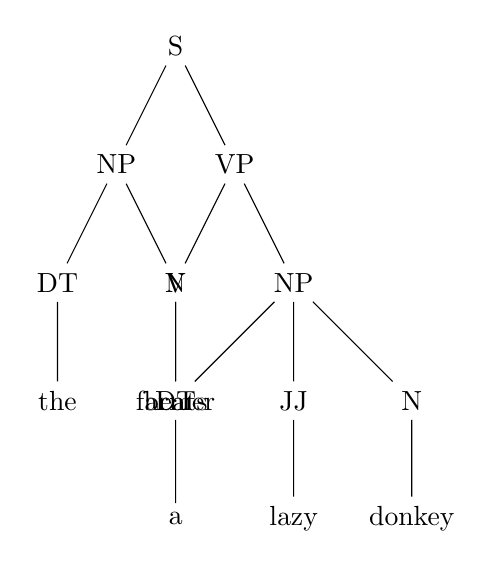
\begin{tikzpicture}[grow=down, sloped]
\node {S}
    child {
        node {NP}
        child {
            node {DT}
            edge from parent
            child {
                node {the}
                edge from parent
            }
        }
        child {
            node {N}
            child {
                node {farmer}
                edge from parent
            }
            edge from parent
        }
        edge from parent
    }
    child {
        node {VP}
        child {
            node {V}
            edge from parent
            child {
                node {beats}
                edge from parent
            }
        }
        child {
            node {NP}
            edge from parent
            child {
                node {DT}
                edge from parent
                child {
                    node {a}
                    edge from parent
                }
            }
            child {
                node {JJ}
                edge from parent
                child {
                    node {lazy}
                    edge from parent
                }
            }
            child {
                node {N}
                edge from parent
                child {
                    node {donkey}
                    edge from parent
                }
            }
        }
        edge from parent
    };
\end{tikzpicture}
\caption{A Constituent Tree} \label{fig:const_tree}
\end{figure}

We will see later how exactly the Montague Grammar obtains a full sentence formula from its reqursive process, but in any case for a computer scientist the introduction of trees is always a promising step.

The main thing to notice now is that for Montague's approach to work, it is crucial that we can always get the meaning of a composed phrase from a composition of the meaning of its subphrases. This compositional property is exactly what we saw earlier that first order logic doesn't posses, and Montague goes through many hoops to simmulate it.

I do however avoid many of those problems, since my goal here is not to test the validity of Montague's proposed rules, but to experiment with how Donkey Monoids and to an extent DPL behaves when put in the framework described. To draw a full circle I am however then going to translate the Donkey Monoids into first order logic so we can easily check if our formulas have the meanings we expect.

This is the chain I am going to build:

\begin{description}
\item[1 Natural Language] We start with a file of simple English natural language sentences. Each line is processed on its own, but may contain more than one sentence.

\item[2 POS tagger] This is the first of three Stanford NLP programs my Haskell script is going to pass the text to. The POS tagger tokenizes the sentences and statstically tries to figures out part of speach for each word. This is our first source of error.

\item[3 Constituent Grammar] It might be that the reason Montague and other early pioneers didn't test their programs mechanically was their lack of access to a good parser. The Stanford Parser is the best on the market, but it still an error rate of around 5\% which is one in every two sentences.

\item[4 Correference Resolution] A lot have been said about how anaphora might be resolved using formal Montague Grammar like approaches. DRT is especially focused on this topic. None the less the current champeon of anaphora competitions\cite{lee2011stanford}\cite{raghunathan2010multi} is the heuristical Stanford Deterministic Coreference Resolution System, the workings of which I will explain in detail.

\item[5 Donkey Monoid] For us the step from 4 to 5 is the most interesting, as it is where we go from syntax to semantics. If we manage to push our original text through to here, not much can go wrong. Only issue is if the logical meaning we create is not the one intended by the speaker.

\item[6 Dynamic Predicate Logic] Since the Donkey Monoids are variants of DPL, they are easy to convert into it. It is much more surprising that DPL lets itself convert into first order logic.

\item[7 First Order Logic] We end up translating our dynamic logics into this old friend. This is mainly done to test the conversion algorithm, and because the first order logic is what we are used to read. The results can be surprising.
\end{description}

However before we can go into the many technical details, we need to develop a very good understanding of the logics and ideas we are working with.

\section{Formal Stuff (10)}

% This should be around 10 pages
%Background should introduce any information that is necessary for the examiner to understand your project. 
%The information here is generally more specific than the background given in the Introduction.
%Requirements gives the program requirements. These chapters prepare the ground for the Design chapter.
%That is: What do we need to handle to be able to solve this problem

In these chapters I'm going to describe the logical theories by Visser and earlier dynamic semantists. I will introduce some addtions of my own and prove interesting properties about them. Finally, but most importantly, I will go into depth with the tools and ideas we need to write a strong logification framework.

In the previous chapter I showed how First Order Logic lack certain compositional properties. A possible solution to this problem is to use a so called `update logic' (a logic with update semantics). Update semantics are logics inspired on the semantics of programming languages where a variable, once introduced, will stick around for a period not know at the time of it's introduction.

The idea of those logics is a `growth of information in time'. Starting from no information, and with each statement adding more. Information is here seen in the information theoretic way, where no information is when everything is possible ($\top$) and total information is when nothing is possible ($\bot$).

Logicians and linguists have come up with many different update logics since the 80s. I will quickly describe the four most cited ones, to give an idea of the landscape we're working in:
%
\begin{itemize}
\item Discourse Representation Theory, 1981 by Hans Kamp\cite{kamp1981theory}, is perhaps the best known approach to using update semantics for understanding language. Kamp takes a very philosophical approach, thinking of his logic as a model for how a person builds up a context during a conversation.

For example, say you you listen to `Some farmer owns no donkey. He beats it'. Discourse Representation Theory (DRT) builds this up from two blocks. Each consists of a set of referents and a set of properties using those. Underlined referents are referents that need to be `merged' with a properly `introduced' one:
%
\begin{align}
&[_1 x\mid farmer(x), \neg[_2 y\mid donkey(y), owns(x,y)] ] \nonumber\\
\oplus\ & [_1 \underline{v}, \underline{w}\mid beats(v,w) ] \nonumber
\end{align}
%
The rule for `$\oplus$' is simply to do a disjoint union of the referents and the properties:
%
\begin{align}
&[_1 x, \underline{v}, \underline{w}\mid farmer(x), \neg[_2 y\mid donkey(y), owns(x,y)], beats(v,w) ] \nonumber
\end{align}
%
At this step it is possible to perform anaphora related heuristics. Since $x$ is the first parameter of $farmer$, we assume it should be so for $beats$ as well:
%
\begin{align}
&[_1 x, \underline{v}, w\mid farmer(x), v=x, \neg[_2 y\mid donkey(y), owns(x,y)], beats(v,w) ] \nonumber\\
&[_1 x, w\mid farmer(x), \neg[_2 y\mid donkey(y), owns(x,y)], beats(x,w) ]\nonumber
\end{align}
%
On the other hand $y$ is not known in the scope of $beats$, so there is no way we can get rid of $w$. And we shouldn't, because in the sentence there is of course no way `it' can refer to `a donkey'.

To deal with our example of `If a farmer owns...', DRT introduces more symbols for weak and strong conditionals.

\item File Change Semantics, 1982 by Irene Heim\cite{heim1983file}, are based around the puzzle of discourse `referents' which may, as we have seen, sometimes act like quantifiers, sometimes referents and sometimes antecedents. Heim suggests using so called `file cards' which though developed independently, has a lot in common with DRT.

However, where DRT defines complex rules for merging different `discourse referents', in File Change Semantics (FCS) the part `added onto' a file gets to decide how the merge is made. Some how similar to how lambda functions in Montague grammars give you a lot of flexibility. For example in case of `adding' $p$, an n-ary atomic predicate, to a file $F$:
%
\begin{align}
&Sat(F + p) = \{a \in Sat(F) \mid R(a_{i_1}, \dots, a_{i_n})\} \nonumber
\end{align}
%
Where $Sat$ is the function that takes a file to the set of `individuals' `satisfying' it.

\item Mental Spaces, 1984 by Fauconnier\cite{fauconnier1984espaces}, is not really a logic in that it's not build on a model theoretic interpretation. It does however build on the same idea of `information growth' on a context representation. Mental Spaces (MS) represent the current context as a graph of predicates and variables:

\tikzstyle{round} = [circle, draw, text width=3em, text centered]
\begin{tikzpicture}[->, >=stealth', semithick, node distance = 3cm, auto]
    % Place nodes
    \node [round] (beats) {beats};
    \node [round, below left of=beats] (x) {x};
    \node [round, left of=x] (farmer) {farmer};
    \node [round, below right of=beats] (z) {z};
    \node [round, right of=z] (donkey) {donkey};
    \node [round, below of=x] (y) {y};
    \node [round, below of=z] (owns) {owns};
    % Draw edges
    \path (beats) edge node {agt} (x);
    \path (beats) edge node {obj} (z);
    \path (z) edge node {dependent} (x);
    \path (z) edge node {a} (donkey);
    \path (x) edge node {every} (farmer);
    \path (x) edge node {def-as} (y);
    \path (owns) edge node {agt} (y);
    \path (owns) edge node {obj} (z);
\end{tikzpicture}

Notice here in particular the interesting the `dependent' arrow. This arrow communicates that there is a one-many relationship between farmer and donkey, and hence that we are talking about a specific donkey for each farmer, not a single poor donkey beaten by everyone.

\item Dynamic Predicate Logic, 1991 by Groenendijk and Stokhof\cite{groenendijk1991dynamic}, is what I will focus on in the remains of this paper. In contrast to some of the previous models, the authors of Dynamic Predicate Logic (DPL) don't make any big philosophical claims on connections between their model and the brain. Instead they simply create a logic that is isomorphic to PL, while keeping a reasonable amount of `update semantics' like properties, such as being closer syntactically to natural language.

DPL also doesn't provide any guidance into resolving anaphora. Just like giving meaning to the actual concepts, this must be handled outside of the logic. We will see later in this paper that this stance makes sense, since the current state of the art anaphora resolvers are simply based on simple heuristics over noun phrases.

In the end of this chapter we will see how a certain monadic construction by Visser can give us as much flexibility in DPL as we would get with a more involved system such as DRT or FCS.
\end{itemize}

\subsection{DPL}

Dynamic Predicate Logic has been developed by a wide group of people: Jan van Eijck and Fer-Jan de Vries\cite{eijck1992dynamic}, Hans Kamp, Veltman, Groenendijk and Stokhof. It is the linguist version of Dynamic Logic invented by Pratt\cite{pratt1976semantical} which is again build on top of Floyd-Hoare Logic for reasoning about computer programs.

The logic cleverly uses these advances in logical understanding to create an update logic in a pragmatic way, without any external constructs and a minimum of new syntax, while still getting all the benefits of compositionality etc.

To model a simple sentence `A man comes in. He sees a donkey. He smiles.', we write:
%
\begin{align}
&(\exists x \cdot man(x) \cdot comes\_in(x)) \nonumber\\
\cdot\ &(\exists y \cdot donkey(y) \cdot sees(x,y)) \nonumber\\
\cdot\ &(smiles(x)) \nonumber
\end{align}

(The parenthesis is only for clarity. The logic is 100\% associative). Notice how we introduce referents casually as we progress in the discourse. We even manage to look pretty similar to PL at the same time. 

Too understand the semantics of the above, let's start by only considering a dynamic propositional logic with three propositions: $P$, $Q$ and $R$. We'll write $p$ to indicate a predicate is true and $\overline{p}$ if it's false. We talked about earlier, that the update semantics modeled `growth of information over time', so we'll start with case that every $2^3$ state is possible:
%
\begin{align}
\{\overline{PQR}, \overline{PQ}R, \overline{P}Q\overline{R}, \overline{P}QR, P\overline{QR}, P\overline{Q}R, PQ\overline{R}, PQR\} \label{dpl_all_states}
\end{align}

Now we'll consider a statement in our predicate logic as a relation between possible states. For example $P\overline{Q}R[P\cdot Q]P\overline{Q}R$ is false, while $P\overline{Q}R[P\cup Q]PQR$ is true. If we take the image of \eqref{dpl_all_states} under $P\cdot\neg Q$ we get
%
\begin{align}
\{P\overline{QR}, P\overline{Q}R\} \label{dpl_PnQ_states}
\end{align}

If we then take the image of \eqref{dpl_PnQ_states} under $\overline{P}$ we end up with the empty set of states. That is there is no possible assignment satisfying our formula, and we consider it a falsum.

The most interesting question is how we work with quantifiers. Which on earth relation could $\exists S$ be? We are going to take a hint from computer programming and consider the variable declaration: $S:=\bot$. We want to write this in DPL as $\exists S \cdot \neg S$, such that e.g. $P\overline{Q}[\exists S \cdot \neg S]P\overline{QS}$ is true. Now since $\cdot\neg S$ acts as a filter, removing all assignments that doesn't have $\overline{S}$, it must be that $\exists S$ is a `random reset, introducing $S$ and allowing it every value, such that $P\overline{Q}[\exists S]P\overline{QS}$ and $P\overline{Q}[\exists S]P\overline{Q}S$ are both true. The image of \eqref{dpl_all_states} under $\exists S$ has 16 possible states.

Let's have a look at the model theoretic definition of the semantics. Visser builds this up in two steps: First a relational algebra and then DPL on top of it. But since DPL is basically identical to the relational algebra, we are going to try and do it in one step.

Let a signature $\Sigma$ for DPL be a structure $\langle Pred, Ar, Var\rangle$. $Pred$ is the set of predicate symbols containing at least $=$, $\top$ and $\bot$. $Ar$ is the function from predicate symbols to their arity and in particular we have $Ar(=) \mapsto 2$, $Ar(\top) \mapsto 0$, $Ar(\bot) \mapsto 0$. Finally $Var$ is the set of variable symbols we may use. We are not going to work with constants in this treatment.

We are further going to define:
%
\begin{align}
Prop_\Sigma &= \{P(x_1,\dots,x_n) \mid P \in Pred,\ Ar(P)=n,\ x_1,\dots,x_n\in Var\}\\
Reset_\Sigma &= \{\exists x \mid x\in Var\}\\
Atom_\Sigma &= Var \cup Prop_\Sigma \cup Reset_\Sigma
\end{align}

A model $\mathcal{M}$ of a signature $\Sigma$ is a tuple $\langle\mathcal{D},\mathcal{I}\rangle$ where $\mathcal{D}$ is a domain which we will always set as $\{\top,\bot\}$, and $\mathcal{I}$ is the interpretation function $Prop_\Sigma\to\mathcal{D}$.

The set of formulas we will say to be the smallest set $Form_\Sigma$ satisfying:
\begin{align}
&Atom_\Sigma \subseteq Form_\Sigma\\
\text{If } \psi\in Form_\Sigma \text{ then } &\neg(\psi)\in Form_\Sigma\\
\text{If } \psi_1,\psi_2\in Form_\Sigma \text{ then } &\psi_1\cdot\psi_2\in Form_\Sigma\\
\text{If } \psi_1,\psi_2\in Form_\Sigma \text{ then } &\psi_1\cup\psi_2\in Form_\Sigma
\end{align}

We are also going to say that an assignment can satisfy a formula, defined as:
\begin{align}
\alpha\models\psi :\equiv \exists\beta(\alpha[\psi]\beta)
\end{align}

Let $[\cdot]$ be the interpretation function from syntax to relation. Then we define the semantics of our logic pointwise for all assignments $\alpha$ and $\beta$:
\begin{align}
\alpha[\psi_1\cdot\psi_2]\beta :\equiv&\ \exists\gamma (\alpha[\psi_1]\gamma \wedge \gamma[\psi_2]\beta) \label{sem_and} \\
\alpha[\psi_1\cup\psi_2]\beta :\equiv&\ \alpha[\psi_1]\beta \vee \alpha[\psi_2]\beta \label{sem_union} \\
\alpha[P(x_1,\dots,x_n)]\beta :\equiv&\ \alpha = \beta \wedge \mathcal{I}(P(\alpha_{x_1},\dots,\alpha_{x_n})) \label{sem_pred} \\
\alpha[\neg\psi]\beta :\equiv&\ \alpha = \beta \wedge \alpha\not\models[\psi] \label{sem_neg}\\
\alpha[\exists x]\beta :\equiv&\ \forall\omega (\omega \neq x \rightarrow \alpha_{\omega} = \beta_{\omega}) \label{sem_exists} \\
\intertext{Using those basic axioms we can derive for our built in propositions:}
\alpha[\bot]\beta \leftrightarrow&\ \alpha = \beta \wedge \bot \nonumber\\
                  \leftrightarrow&\ \bot \label{sem_bot}\\
\alpha[\top]\beta \leftrightarrow&\ \alpha = \beta \wedge \top \nonumber\\
                  \leftrightarrow&\ \alpha = \beta \label{sem_top}\\
\intertext{Taking $\psi_1\rightarrow\psi_2$ to mean $\neg(\psi_1\wedge\neg\psi_2)$ we also get the following neat equation, originally by Groenendijk and Stokhof\cite{groenendijk1991dynamic}:}
\alpha[\psi_1\rightarrow\psi_2]\beta
 :\equiv&\ \alpha[\neg(\psi_1\wedge\neg\psi_2)]\beta \nonumber\\
 \leftrightarrow&\ \alpha = \beta \wedge \alpha\not\models[\psi_1\wedge\neg\psi_2] \nonumber\\
 \leftrightarrow&\ \alpha = \beta \wedge \neg\exists\gamma(\alpha[\psi_1\wedge\neg\psi_2]\gamma) \nonumber\\
 \leftrightarrow&\ \alpha = \beta \wedge \neg\exists\gamma(\exists\delta(\alpha[\psi_1]\delta\wedge\delta[\neg\psi_2]\gamma)) \nonumber\\
 \leftrightarrow&\ \alpha = \beta \wedge \neg\exists\gamma(\exists\delta(\alpha[\psi_1]\delta\wedge\delta=\gamma\wedge\delta\not\models[\psi_2])) \nonumber\\
 \leftrightarrow&\ \alpha = \beta \wedge \forall\gamma(\forall\delta(\delta=\gamma\rightarrow(\alpha[\psi_1]\delta\rightarrow\delta\models[\psi_2]))) \nonumber\\
 \leftrightarrow&\ \alpha = \beta \wedge \forall\gamma(\alpha[\psi_1]\gamma\rightarrow\gamma\models[\psi_2]) \label{sem_impl}
\end{align}

In my implementation section, I describe how the above can be efficiently implemented in Haskell using an isomorphism between relations $\mathcal{P}(A\times B)$ and functions $A\to\mathcal{P}(B)$. I also show how the kleiski combinator takes the role of $\cdot$.

However let's first look at some of the implications of the above definitions. For example, how can we intuitively understand the DPL notion of $\rightarrow$? Well, first notice that many of the equations start with $\alpha=\beta\wedge\dots$. These equations we can think of intuitively as having a closed scope. We saw earlier how DRT nicely determined that the `it' in `A farmer doesn't own a donkey. He beats it' couldn't refer to `a donkey' because the negation didn't let it's variable out. In DPL we get the same effect. Because an assignment must be the same before and after a negated clause, all new variables introduced inside the clause have disappeared.

Of course this `static negation' might not always be the right thing. Consider the sentences `It is not that case that a farmer doesn't own a donkey. He beats it'. This should be a good sentence, but we can't handle it. In the next chapter we will look at how this might be handled.

The DPL $\psi_1\rightarrow\psi_2$ in particular can be seen as the filter, that if you can get `through' $\psi_1$ then you must also be able to get through $\psi_2$. But notice that $\gamma$ doesn't have to equal $\alpha$. Hence variables introduced in $\psi_1$ can well bind variables in $\psi_2$. This will show to be extremely important in the treatment of donkey sentences later.

Talking about binding, also notice that our union or `or' construct is a bit special. $\psi_1$ and $\psi_2$ cannot bind variables in each other, but in $(\psi_1\cup\psi_2)\cdot\psi_3$ they can both bind variables in $\psi_3$. This is going to introduce a lot of weird situations later. In the next section we will look closer at these problems, and also consider the alternative definition of `or': $\neg(\neg\psi_1\cdot\neg\psi_2)$.

\subsubsection{The problem with disjunction}

We won't actually use `or' in the implementation.
Example of the problems we still have in the logic.
Can't tell what variables are available where.

A major problem with our use of `relation union' as disjunction is the way it allows seemingly sound sentences to combine into syntactically invalid ones. Consider the sentence `Either a farmer owns a donkey or he doesn't'. We would write that as
\begin{align}
\exists x\cdot farmer(x)\cdot(\exists y\cdot owns(x,y)\cdot donkey(y)\vee \bot) \label{owns_donkey_or_not}
\end{align}
Now concatenating this sentence with `he beats it': $beat(x,y)$ would give us a problem. In fact this problem would be more than a syntactic problem, because before we know the model and the existence of the donkey, we don't know if the sentence is valid or not.

Visser\cite{visser1999donkey} suggests that we should build our logic on sets of relations read disjunctively instead of just relations. This `possible world' scenario would transform \eqref{owns_donkey_or_not}$\cdot beats(x,y)$ into $\{\exists x\cdot farmer(x)\cdot\exists y\cdot donkey(y)\cdot owns(x,y)\cdot beats(x,y), \exists x\cdot farmer(x)\cdot\bot\cdot beats(x,y)\} = \{\exists x\cdot farmer(x)\cdot\exists y\cdot donkey(y)\cdot owns(x,y)\cdot beats(x,y), \bot\}$. This clearly is always well defined.

Visser's idea doesn't fully save us though. If we now consider `a farmer either owns a donkey or owns a horse':
\begin{align}
\exists x\cdot farmer(x)\cdot(&\exists y\cdot owns(x,y)\cdot donkey(y)\nonumber\\
                              &\vee \exists z\cdot owns(x,z)\cdot horse(z))
\end{align}
And combines that with `He beats the donkey': $beat(x,y)$, we get, in Visser's model, $\{\exists x\cdot farmer(x)\cdot\exists y\cdot owns(x,y)\cdot donkey(y)\cdot beats(x,y), \exists x\cdot farmer(x)\cdot\exists z\cdot owns(x,z)\cdot horse(z)\cdot beats(x,y)\}$. The second one is clearly not valid (though we wouldn't get a problem if there is no horse or farmer) which we might catch `at compile time' and replace it with something like `$\bot$' or `error'. This sort of error handling is discussed and implemented in the implementation section, but is not terribly interesting from a formal point of view.

Much more interesting are the following two questions: How could we have translated \label{owns_donkey_or_horse} so it would actually work? After all it seemed like a reasonable sentence until variable naming got us. And does the way variable binding works with our definition actually make sense?

Clearly just renaming $z$ to $y$ in the horse term would have solved the first problem. However to work in a compositional way, that would either require great luck, or renaming, and we don't have a renaming operator.

A trick we could consider is to declare an `object' variable outside of the disjunction:
\begin{align}
\exists s\cdot farmer(s)\cdot\exists o\cdot(
      &\exists y\cdot owns(s,y)\cdot donkey(y)\cdot o=y \nonumber\\
      &\vee \exists z\cdot owns(s,z)\cdot horse(z)\cdot o=z)\cdot beats(s,o)
\end{align}
%
This even inspires on idea that we might be able to build everything up around subjects, objects, indirect objects etc. This is explored in the implementation, but it does suffer from many problems. E.g. we might well have a sentence very similar to the above: `A farmer owns a donkey and owns a horse. He beat them'. Here we suddenly have two objects in the same sentence.

Sentences like the above are easy to make in English because the absence of noun genders make it easy to use the same pronoun to refer to a lot of things at once. By choosing the right actors however, it is always possible to run into problems.

The problem is perhaps the non-linearity in the way variables pass through the disjunction. Somehow we lose track of their history when the `results' are merged together.

This leads on to the other question we mentioned: Is the binding flow through our disjunction operator really any good? We are is inspired by the sentence `Either a farmer or his scapegoat must go to court. In any case he will be picked up by sunset'. In terms of DPL formulas, this would be modelled something like $(\psi_1\cup\psi_2)\cdot\psi_3$. Clearly we have a problem here: Variables bound in $\psi_1$ are not accessible in $\psi_2$.

This sentence suggests that we might want to define a disjunction operator with a linear flow of variables: $\psi_1\to\psi_2\to\psi_3$ instead of $\psi_1\to\psi_3\text{ and }\psi_2\to\psi_3$. However there is a problem: We currently define `false' as the absence of possible assignments. Hence if $\psi_1$ is false, there is no way we can define disjunction to push it's variables into $\psi_2$. If any variables were left undefined, $\psi_1$ wouldn't be false.

There is a cure to this problem. When we extend our logic with more power in the monad chapter, we get a second chance. However Let's first have a look at an obvious alternative definition for disjunction considered by Groenendijk\cite{groenendijk1991dynamic}. We'll call it `static disjunction':
\begin{align}
\alpha[\psi_1\vee\psi_2]\beta
 :\equiv&\ \alpha[\neg(\neg\psi_1\wedge\neg\psi_2)]\beta \nonumber\\
 \leftrightarrow&\ \alpha[\neg\psi_1\rightarrow\psi_2]\beta \nonumber\\
 \leftrightarrow&\ \alpha = \beta \wedge \forall\gamma(\alpha[\neg\psi_1]\gamma\rightarrow\gamma\models[\psi_2]) \nonumber\\
 \leftrightarrow&\ \alpha = \beta \wedge \forall\gamma((\alpha=\gamma\wedge\gamma\not\models\psi_1)\rightarrow\gamma\models[\psi_2]) \nonumber\\
 \leftrightarrow&\ \alpha = \beta \wedge \forall\gamma(\alpha=\gamma\rightarrow(\gamma\models\psi_1\vee\gamma\models\psi_2)) \nonumber\\
 \leftrightarrow&\ \alpha = \beta \wedge (\alpha\models\psi_1\vee\alpha\models\psi_2) \label{sem_or}
\end{align}

The idea to this follows natural from De Morgan's laws of classical logic. Clearly the semantics are different from the ones we defined for $\cup$. However not in a good way. This static disjunction doesn't allow any variables to escape from inside it's reach.

So does this fix our problem of binding between clauses? No. In fact this definition doesn't even allow binding from a clause and out. The villain is $\neg\psi$. From the first mention we defined it to be static so it wouldn't allow unsafe, arbitrary assignments as long as they didn't satisfy $\psi$. We wanted our logic to be reasonably monotonic, and we got what we deserved. $\neg$ not only closed down this version of disjunction, but our implication definition as well.

We can imagine defining $\neg$ dynamically: $\neg\psi_1\cdot\psi_2 = \neg(\psi_1\cdot\psi_2)$. However not in our current model, and it won't solve any of our problems with disjunction. It does however allow this sentence: `It is not the case that a farmer doesn't own a donkey. He beats it'. While it made sense not to allow variables to escape from a single $\neg$, we want them to escape from a double.

\subsubsection{Connection with first order logic}

An interesting property of DPL is that it is isomorphic with classical logic. Any PL formula corresponds to one in DPL and vice versa. This gives an alternative way to define and understand the semantics of DPL, and it relaxes us that nothing `weird' is going on. We might also be a bit disappointed that after all this, we don't possess any extra power, but let's forget about that for now, and see how the conversion works.

Let $\phi$ be a formula in negation normal form, or something. Hmm, come back here once the disjunction chapter is done.
\begin{align}
&[\exists x(\phi)] \equiv \neg(\neg(\exists x \cdot [\phi]))\\
&[\forall x(\phi)] \equiv \exists x \rightarrow [\phi]\\
&[\phi_1\wedge\phi_2] \equiv [\phi_1]\cdot[\phi_2]\\
&[\phi_1\vee\phi_2] \equiv \dots\\
&[\neg(\exists x)] \equiv \dots\\
&[\neg(\phi_1\wedge\phi_2)] \equiv \neg[\phi_1]\cdot\neg[\phi_2]\\
&[\neg(\phi_1\vee\phi_2)] \equiv \dots
\end{align}

Similarly we may create PL formulas with the same meaning as any DPL formula. But perhaps we should be a bit concerned on how to interpret the meaning of a PL formula and a DPL formula being equivalent. After all DPL formulas are relations where PL formulas a propositions. In the above it was all easy, but let's think again about what we are doing.

Remember that we said an assignment could model a DPL relation. If we consider the truth value of a DPL relation to be whether there exists any relation that models it $\exists\alpha(\alpha\models\psi)$, we can use a trick. The trick is to think of the weakest precondition such an assignment must satisfy, and model that in PL. In fact the precondition is not just for our assignment, but for the entire model. For example to model $\exists x\cdot farmer(x)$ the starting assignment might well be empty ($\bot$), but our model must contain an entity for which $farmer$ is true.

To smoothen the following derivations, we will introduce a special syntax `$\langle\psi\rangle\phi$' where $\psi$ is a DRA formula, $\phi$ is a PL formula and the whole thing is a PL formula. For some assignment $\alpha$, we define `$\alpha\models\langle\psi\rangle\phi$' to mean $\exists\beta(\alpha[\psi]\beta \wedge \beta\models\phi)$.
%
\begin{align}
\alpha\models\langle\exists x\rangle\phi
 & \leftrightarrow \alpha\models\exists x (\phi) \label{conv_exists}\\
\alpha\models\langle\psi_1\cdot\psi_2\rangle\phi
 & \leftrightarrow \alpha\models\langle\psi_1\rangle\langle\psi_2\rangle\phi \label{conv_and}\\
\alpha\models\langle\psi_1 \cup \psi_2\rangle\phi
 & \leftrightarrow \alpha\models\langle\psi_1\rangle\phi \vee \langle\psi_2\rangle\phi \label{conv_or}\\
 \alpha\models\langle\psi_1 \vee \psi_2\rangle\phi
\alpha\models\langle P(x_1,\dots,x_n)\rangle\phi
 & \leftrightarrow \alpha\models P(x_1,\dots,x_n) \wedge \phi \label{conv_pred}\\
\alpha\models\langle\neg\psi\rangle\phi
 & \leftrightarrow \alpha\models \neg\langle\psi\rangle\top \wedge \phi \label{conv_neg}
\end{align}

See the appendix for my full derivations of every equation. Also notice that $\alpha\models\langle\bot\rangle\phi\leftrightarrow a\models\bot$ and $\alpha\models\langle\top\rangle\phi\leftrightarrow a\models\phi$ follow trivially from \eqref{conv_pred}. Equations for `convenience' operators such as $\rightarrow$ and $\vee$ can be derived too:
\begin{align}
\langle\psi_1\vee\psi_2\rangle\phi
& \leftrightarrow \langle\neg(\neg\psi_1\cdot\neg\psi_2)\rangle\phi \nonumber\\
& \leftrightarrow \neg\langle\neg\psi_1\cdot\neg\psi_2\rangle\top \wedge\phi \nonumber\\
& \leftrightarrow \neg\langle\neg\psi_1\rangle\langle\neg\psi_2\rangle\top \wedge\phi \nonumber\\
& \leftrightarrow \neg\langle\neg\psi_1\rangle(\neg\langle\psi_2\rangle\top) \wedge\phi \nonumber\\
& \leftrightarrow \neg(\neg\langle\psi_1\rangle\top \wedge \neg\langle\psi_2\rangle\top) \wedge\phi \nonumber\\
& \leftrightarrow (\langle\psi_1\rangle\top \vee \langle\psi_2\rangle\top) \wedge\phi \label{conv_vee}
\end{align}

In the implementation we will use the above equations to recursively convert our DPL formulas to PL. The $\langle\rangle$ notation easily lends itself to calculation by a stack manipulation function.

The rules will look like:
\begin{haskell}
addDpl :: Prop -> [DPL] -> Prop
addDpl p ((DNot d):ds) = addDpl (And (Not (addDpl T [d])) p) ds
\end{haskell}


\subsection{Donkey Monoids}

Imagine translating this sentence to DPL:
%
\begin{quotation}
A farmer owns a donkey, if he beats it
\end{quotation}
%
We would have to write something along the lines of:
%
\begin{equation}
\exists x \cdot farmer(x) \cdot \exists y \cdot donkey(y) \cdot beats(x,y) \rightarrow owns(x,y)
\end{equation}
%
The problem here is that reorderings like this work against our sought property of linearity: of being able to add new information as we go. We cannot compose `A farmer owns a donkey' and `if he beats it' in a meaningful way.

To rescue us from this problem Albert Visser suggests constructing a special e-monoid over the dynamic relational algebra. The idea is that we are going to simultaneously work on two `streams' of dpl, and switch easily between them with a special element $\Bowtie$.

Our sentence from above will then be expressible as
%
\begin{equation}
\Bowtie \cdot \exists x \cdot farmer(x) \cdot \exists y \cdot donkey(y) \cdot \Bowtie \cdot owns(x,y) \cdot \Bowtie \cdot beats(x,y)
\end{equation}
%
which can be written in `stream form' as
%
\begin{equation}
\begin{tabular}{|clll|}
    \hline
    $(-)$ & $\exists x \cdot farmer(x) \cdot \exists y \cdot donkey(y)$ & ~ & $beats(x,y)$ \\\hline
    $(+)$ & ~ & $owns(x,y)$ & ~ \\\hline
\end{tabular}
\end{equation}
%
The meaning of the above is $(-) \rightarrow (+)$

Another example from Visser is:
\begin{quotation}
A man keeps his word. He is honest
\end{quotation}
which roughly translates to:
\begin{equation}
\Bowtie\cdot\exists x\cdot man(x)\cdot\Bowtie\cdot keepword(x)\cdot honest(x)
\end{equation}
If you are interested in a lot more examples, see Visser's paper\cite{visser1999donkey}.

So how do we define this nifty $\Bowtie$? The trick is to move the entire dynamic relation algebra from before into an e-monoid that will help us keep track of some details.

If $\phi$ from before is the basic algebra, we specify the construction of our monoid $\Phi$ as follows.
%
\begin{flalign}
&\top := \langle \top, \top, + \rangle & \\
&\bot := \langle \top, \bot, + \rangle & \\
&\Bowtie := \langle \top, \top, - \rangle & \\
&\langle q_-, q_+, \alpha \rangle \cdot \langle r_-, r_+, \beta \rangle := \langle q_- \cdot r_{-\alpha}, q_+ \cdot r_{+\alpha}, \alpha\beta \rangle&
\end{flalign}
%
Notice how we keep the negative stream in the first position of the tuple, and the positive stream at the second position. The third position indicates to what stream we are currently writing. For example, if we are writing to the negative stream, and we apply an element that itself asks us to continue at its negative stream, we go back to the positive stream.

An even more interesting element than $\Bowtie$ is $\triangle$. $\triangle$ is a scope modifier, and it allows us to write:
%
\begin{quote}
A farmer owns a donkey. He beats it.
\end{quote}
%
(that is just some single farmer and donkey) as
%
\begin{equation}
\triangle \cdot \exists x \cdot farmer(x) \cdot \triangle \cdot owns(x,y) \cdot \triangle \cdot \exists y \cdot donkey(y) \cdot \triangle \cdot beats(x,y)
\end{equation}
%
That is very close to the order of the natural language!

And combining the two monads we can do our original sentence as
%
\begin{quote}
If a farmer owns a donkey, he beats it
\end{quote}
%
as
\begin{equation}
\Bowtie \cdot \triangle \cdot \exists x \cdot farmer(x) \cdot \triangle \cdot owns(x,y) \cdot \triangle \cdot \exists y \cdot donkey(y) \cdot \triangle \cdot \Bowtie \cdot beats(x,y)
\end{equation}
%
In stream form, that is:
%
\begin{equation}
\begin{tabular}{|cllll|}
    \hline
    $(-,1)$ & $\exists x \cdot farmer(x)$ & ~ & ~ $ \exists y \cdot donkey(y)$ & ~ \\\hline
    $(-,0)$ & ~ & $owns(x,y)$ & ~ & ~ \\\hline
    $(+,1)$ & ~ & ~ & ~ & ~ \\\hline
    $(+,0)$ & ~ & ~ & ~ & $beats(x,y)$ \\\hline
\end{tabular}
\end{equation}
%
With the meaning being $(-,1) \cdot (-,0) \rightarrow (+,1) \cdot (+,0)$. Notice that the negative relations are again put on the left side of the implication, and the relations with larger scope value are put before those of lower value.

Notice $\Bowtie$ and $\triangle$ are commutative, since they work entirely on their own indicator. It's an interesting question to consider what sentences might require three or more levels of scoping. We could define $\triangle$ to go up in scope and $\bigtriangledown$ to go down. Instead of ${0,1}$ we would work on $\mathbb{Z}$.

For now we define the monad as follows:
%
\begin{flalign}
&\top := \langle \top, \top, \top, \top, +, 0 \rangle & \\
&\bot := \langle \top, \top, \top, \bot, +, 0 \rangle & \\
&\Bowtie := \langle \top, \top, \top, \top -, 0 \rangle & \\
&\triangle := \langle \top, \top, \top, \top +, 1 \rangle & \\
&\langle q_{-,1}, q_{-,0}, q_{+,1}, q_{+,0}, \alpha, i \rangle \cdot \langle r_{-,1}, r_{-,0}, r_{+,1}, r_{+,0}, \beta, j \rangle := &\\
&\hspace{1cm}\langle q_{-,1} \cdot r_{-\alpha,1+i}, q_{-,0} \cdot r_{-\alpha,i}, q_{+,1} \cdot r_{\alpha,1+i}, q_{+,0} \cdot r_{\alpha,i}, \alpha\beta, i+j \rangle& \nonumber
\end{flalign}

In his paper Visser now goes on to define $\triangleleft$ and $\triangleright$ which work similarly to $\Bowtie$ except they work in different directions. 
%
\begin{equation}
\Bowtie \cdot \triangle \cdot \exists x \cdot farmer(x) \cdot \triangle \cdot owns(x,y) \cdot \triangle \cdot \exists y \cdot donkey(y) \cdot \triangle \cdot \triangleleft \cdot beats(x,y)
\end{equation}
%
This is quite interesting for certain sentences containing `surprises', like
%
\begin{quotation}
He sees... no donkey
\end{quotation}
%
In this case we would compositionally assume to start out with
$sees(x,y)$ and finish with $\cdot \exists y \cdot donkey(y)\triangle$ hence we want to write something like:
%
\begin{equation}
sees(x,y) \cdot \triangleleft \cdot \bot \cdot \triangleright \cdot \triangle \cdot \exists y \cdot donkey(y) \cdot \triangle
\end{equation}
%
Notice that that means the word `no'/`not' must be $\triangleleft\cdot\bot\cdot\triangleright$. Unfortunately these retrospective triangles tend to mess sentence enough up, that they require lots of `stream unification brackets', and don't generally give very nice formulas. In the semantic parsing in the next section, they wont be used at all.

\subsection{Montague Semantics}
Montague semantics is a theory of natural language that believes its semantics can be described thoroughly in terms of standard mathematical models. Logician Richard Montague (1930-1971) famously wrote
\begin{quotation}
There is in my opinion no important theoretical difference between natural languages and the artificial languages of logicians; indeed I consider it possible to comprehend the syntax and semantics of both kinds of languages with a single natural and mathematically precise theory. \cite{montague1970universal}
\end{quotation}

He believed that just as Chomsky had formulated the syntax of language in a mathematical framework, so too should it be possible to define the meaning of every sentence, based on the meaning of its parts and a set of compositional rules.

While the above remains a hot topic in the philosophy of language, we are going to take a more practical stand. In our quest to automate the translation of language into Visser's monadic DPL, it is interesting that Montague was able to define such a large fragment of English using familiar tools of compositionality and lambda calculus.

The basic idea is very simple. For each postag we define a type. E.g. $S$ has the type $Bool$ and $VP$ has the type $Entity \rightarrow Bool$, the intuition being that the VP returns true if the entity `does what the VP described' and false otherwise. An NP is given type type $VP \rightarrow Bool$ which allows it to create a scope for a variable and pass it to the VP, or whatever it sees fitting for that NP.

The point is that we always give a specific phrase type the same logical type. This allows our composition rules to know exactly what type each component has. Here are some more examples:
\begin{itemize}
\item Proper noun (John, Oxford): Entity
\item One-place predicate constant (farmer, sleeps, walks): $Entity \rightarrow Bool$
\item Transitive verb (owns, beats): $Entity \rightarrow Entity \rightarrow Bool$
\item Attributive adjective (good, intelligent, former): $(Entity \rightarrow Bool) \rightarrow (Entity \rightarrow Bool)$
\item Quantifiers/Determiners (a, the, every, no): $(Entity \rightarrow Bool) \rightarrow (Entity \rightarrow Bool) \rightarrow Bool$
\end{itemize}

To translate a sentence like `Every farmer beats a donkey' we first create a constituent tree [$_\text{S}$ [$_\text{NP}$ [$_\text{DT}$ Every] [$_\text{NN}$ farmer]] [$_\text{VP}$ [$_\text{VBZ}$ beats] [$_\text{NP}$ [$_\text{DT}$ a] [$_\text{NN}$ donkey]]]].

Next we create objects for the basic elements (a computer would do this recursively, but it is easier for us to do it level by level):
\begin{equation*}\begin{aligned}
&\text{Every, $r_1$}=&& \lambda xy(\Bowtie\cdot\triangle\cdot\exists r_1\cdot (xr_1)\cdot\triangle\cdot\Bowtie\cdot (yr_1)) &&:: (E\rightarrow B)\rightarrow(E\rightarrow B)\rightarrow B\\
&\text{farmer}=&& \lambda x(farmer(x)) &&:: E\rightarrow B\\
&\text{beats}=&& \lambda xy(beats(xy)) &&:: E\rightarrow E\rightarrow B\\
&\text{a, $r_2$}=&& \lambda xy(\triangle\cdot\exists r_2\cdot (xr_2)\cdot\triangle\cdot (yr_2)) &&:: (E\rightarrow B)\rightarrow(E\rightarrow B)\rightarrow B\\
&\text{donkey}=&& \lambda x(donkey(x)) &&:: E\rightarrow B\\
\midrule
&\text{Every farmer}=&& \lambda y(\Bowtie\cdot\triangle\cdot\exists r_1\cdot farmer(r_1)\cdot\triangle\cdot\Bowtie\cdot (yr_1)) &&:: (E\rightarrow B)\rightarrow B\\
&\text{a donkey}=&& \lambda y(\triangle\cdot\exists r_2\cdot donkey(r_2)\cdot\triangle\cdot (yr_2)) &&:: (E\rightarrow B)\rightarrow B\\
\midrule
&\text{beats a donkey}=&& \lambda z(\triangle\cdot\exists r_2\cdot donkey(r)\cdot\triangle\cdot beats(z,r_2)) &&:: E\rightarrow B\\
\end{aligned}\end{equation*}

Until we can then finally compose the top NP and VP to get the sentence:
\begin{equation*}\begin{aligned}
&\Bowtie\cdot\triangle\cdot\exists r_1\cdot farmer(r_1)\cdot\triangle\cdot\Bowtie\cdot \triangle\cdot\exists r_2\cdot donkey(r_2)\cdot\triangle\cdot beats(r_1,r_2)\\
=\text{ }&\Bowtie\cdot\triangle\cdot\exists r_1\cdot farmer(r_1)\cdot\triangle\cdot\Bowtie\cdot beats(r_1,r_2)\cdot \triangle\cdot\exists r_2\cdot donkey(r_2)\cdot\triangle
\end{aligned}\end{equation*}

You might have noticed we didn't discuss how the variables $r_1$ and $r_2$ were assigned. This is of course of utter importance in relation to anaphora resolution. However in the section \ref{sec:coreferences} we will discuss a way out of this problem.

Later in the implementation section we will look at more issues regarding to using Montague Grammars in practise. First we need to look at a very important source of ambiguity in sentences.

\subsubsection{Weak and strong readings}

`Weak' and `strong' are quite accepted terms in linguistics for describing different ways to interprete quantifiers. In line with information theory, we can say that weak readings are about weak information and strong readings about strong information.

Makoto Kanazawa has written an entire paper on issues with weak and strong readings of donkey sentences\cite{kanazawa1994weak}. For the donkey sentence, we may have at least the following readings of the second `a':
\begin{enumerate}
\item Weak reading: A farmer who owns a donkey beats a donkey he owns. 
\item Strong reading: A farmer who owns a donkey beats every donkey he owns 
\item Unique reading: A farmer who owns a donkey beats the donkey he owns. 
\end{enumerate}

We have equally many reaings for the first `A', creating nine possible interpretations. This is because `a' is a very ambigious quantifier. Other quantifiers such as `every' and `all' are more clearly defined. `Some' is another example of an ambigious quantifier.

Often we can use the context of a sentence to determine which meaning is the correct one. For example:
\begin{quotation}
Every farmer owns a donkey. It is pink.
\end{quotation}
Here it is clear that all the farmers share one donkey. Hence perhaps the best solution to the problem is to generate all possible sentences and let the context decide which ones survive.

\subsection{Dependency Graphs}

\tikzstyle{level 1}=[level distance=2cm, sibling distance=3.5cm]
\tikzstyle{level 2}=[level distance=2.5cm, sibling distance=3.5cm]
\tikzstyle{level 3}=[level distance=2cm, sibling distance=3.5cm]
\begin{figure}
\centering
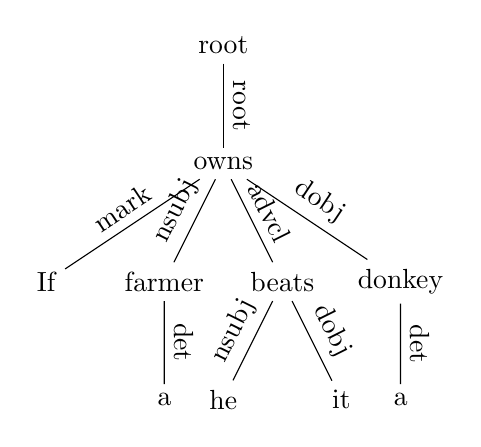
\begin{tikzpicture}[grow=down, sloped]
\node {root}
    child {
        node {owns}
        child {
            node {If}
            edge from parent
            node[above] {mark}
        }
        child {
            node {farmer}
            child {
                node {a}
                edge from parent
                node[above] {det}
            }
            edge from parent
            node[above] {nsubj}
        }
        child {
            node {beats}
            child {
                node {he}
                edge from parent
                node[above] {nsubj}
            }
            child {
                node {it}
                edge from parent
                node[above] {dobj}
            }
            edge from parent
            node[above] {advcl}
        }
        child {
            node {donkey}
            child {
                node {a}
                edge from parent
                node[above] {det}
            }
            edge from parent
            node[above] {dobj}
        }
        edge from parent
        node[above] {root}
    };
\end{tikzpicture}
\caption{Dependency graph for `If a farmer owns a donkey, he beats it'} \label{fig:dependency_graph}
\end{figure}

Dependency graphs are an alternative way of parsing sentences. Where constituent trees keep the original word order, dependency graphs are allowed to move thing around in any way they like\footnote{Until now we've been lucky that things next to each other often were related, but in some languages other than English, words can jump anywhere they like, and our approach might fail.}. Also dependency graphs don't have to be trees.

The flexibility of dependency graphs allow them to do a lot of interesting things. In our favourite example of the donkey and the farmer we had the problem that there wasn't a very strong syntactical relationship between `farmer' and `he'. In figure \ref{fig:dependency_graph} we see how the same sentence would look if parsed with a dependency parser.

The first thing we notice is that dependency graphs focus on verbs. The verbs become the heads of the sentences, and everything else becomes the ` subject', `the object' or `the something else' of the verb. In our example `he beats it' becomes an `adverbial clause modifier' of the main verb. This means it modifies the verb, here in the sence of making the main verb a condition.

Dependency graphs naturally seems to offer more semantic information than constituent trees, and hence that they would be a good intermediate step towards our goal of logification. However the first disappointment arrise as we start to look at how they are created.

The Stanford Parser makes dependency graphs using a special kind of regular expressions for trees called `tregex'\cite{de2006generating}. It defines tregex rules such as:
%
\begin{equation}
NP < NN\ \$\ VP
\end{equation}
Which means an NP that is the parent of an NN and sister of a VP.

Another more complicated example is:
\begin{equation}
NP < (NN < dog)\ \$\ (VP <\!\!<\# (barks > VBZ))
\end{equation}
Which means an NP over an NN over `dog' and with a sister VP headed by `barks' which is a verb in present singular.

Obviously this means we can't get any information from the graph that we couldn't also get from the tree. In fact it probably contains less. On the flip side however, the regular expressions are clearly more powerful than simple recursions as we define them in the Montague grammars.

I've worked hard on trying to define a Montague like set of equations for Enlish, but over the dependency graph. This has however failed, mostly due to one simple reason: In a Montague grammar we expect every type of phrase to have a specific logical type. E.g. all NPs are `VP $\rightarrow$ Bool' and VPs are `Entity $\rightarrow$ Bool'. This makes it fit very nice in a programming context, where we can define a function `parseNP :: ConstituentTree $\rightarrow$ (VP $\rightarrow$ Bool)'. With the dependency approach we don't have this option. A `subj' arrow can mean many different things. Sometimes it points at a noun, sometimes at a proper noun, sometimes something else.

In conclusion, Montague like grammars for dependency graphs could be very interesting to make. It would however require some welldefined rules for what we can expect to find under each type of arrow. This was a blind road.

\subsection{Coreferences}\label{sec:coreferences}
Coreferences (or anaphora) is essential in order to create advanced discourse, since it is what allows us maintain a topic beyond the first mention. Without coreferences we couldn't even express simple logical statements such as transitivity: `a man's brother's brother is his brother' etc.

Identifying coreferences (or resolving anaphora) is hence an important part of converting natural language into logic. The issue is not touched upon in Visser's paper, which casually sidesteps the problem by assigning variables to all mentioned entities.

For the subtask of resolving simple pronouns a solution could be to work in terms of subjects, objects, indirect objects and so on. However if not earlier, this certainly fails for pronouns separated from their antecedent by sentence boundaries. Also we want to resolve other kinds of coreferences, such as `John, the farmer, owns a donkey', where `the farmer' and `John' refers to the same entity.

It quickly becomes clear that the problem is not only syntactical. In the sentence `John and his wife had a farm. He took care of the donkeys' we could substitute `He' with `She' and to change the referent of the pronoun. In this case we need semantic knowledge of genders to proceed.

In my project I have taken advantage of the coreference tagger built into Stanford CoreNLP\cite{lee2013deterministic}\cite{lee2011stanford}\cite{raghunathan2010multi}. In the following section I will summarize the workings of this machine, made to work across large texts as well as simple sentences.

Coreference tagging is one part of computational linguistics where machine learning algorithms still haven't been able to outperform large iterative applications of linguistic heuristics. Of course the procedure assumes (most likely) machine learned postagging and named entity recognition, but the main algorithm is transparent and deterministic.

The idea is to iteratively go over the text with different `sieves'. The below example explains each step with an example I have adopted from \cite{lee2013deterministic}:

\begin{quotation}
John is a farmer. He owned a stubborn donkey.
A girl was looking at the donkey.
``It was my favorite,'' John said to her.
\end{quotation}

\begin{description}
\item[Mention detection]
The first step is to identify all noun phrases (NP) and personal (PRP) and possessive (PRP\$) pronouns. This information is easily pulled from the constituent tree. Notice we also identify nested mentions:

[John]$_1^1$ is [a farmer]$_2^2$. [He]$_3^3$ owned [a stubborn donkey]$_4^4$.\newline
[A girl]$_5^5$ was looking at [the donkey]$_6^6$.\newline
``[It]$_7^7$ was [[my]$_9^9$ favorite]$_8^8$,'' [John]$_{10}^{10}$ said to [her]$_{11}^{11}$.

All mentions are initially assigned to separate entities (entity ids). The entities are also attached information we can easily pull from the constituent tree, such as `a girl: {number: singular, gender: female}' which are used for the following rules.
\item[Speaker Sieve]
The purpose of this first sieve is to link self referring pronouns to speakers. Speakers are identified simply by their connection to verbs such as `say' and proximity to the quotations. In our case the pronoun `my' gets linked to `John':

[John]$_1^1$ is [a farmer]$_2^2$. [He]$_3^3$ owned [a stubborn donkey]$_4^4$.\newline
[A girl]$_5^5$ was looking at [the donkey]$_6^6$.\newline
``[It]$_7^7$ was [\textbf{[my]$_9^1$} favorite]$_8^8$,'' \textbf{[John]$_{10}^{9}$} said to [her]$_{11}^{11}$.

In conversational text we would store information about the speakers in our entities. Thus we could e.g. match mentions of `you' to the speaker of the previous quote we saw.

We also note restrictions for future use, so we don't risk coreferencing an `I' with a `he' etc.
\item[String Match]
The second step is to merge entities referred to by exactly the same string. In our case we have two mentions of `John':

\textbf{[John]$_1^1$} is [a farmer]$_2^2$. [He]$_3^3$ owned [a stubborn donkey]$_4^4$.\newline
[A girl]$_5^5$ was looking at [the donkey]$_6^6$.\newline
``[It]$_7^7$ was [[my]$_9^1$ favorite]$_8^8$,'' \textbf{[John]$_{10}^{1}$} said to [her]$_{11}^{11}$.
\item[Relaxed String Match]
This third sieve doesn't get activated by our example. It will try to remove relative clauses and other text following the head word of a mention, and do an exact match of the result. For example [John] and [John, whose donkey loves him] will correctly be merged.

Like the `String Match' sieve, we are not doing anything fancy here, and we will incorrectly coreference the two mentions of `John' in: `[John, who loves donkeys] and [John, who hates donkeys] were brothers.'
\item[Precise Constructs]
The `Precise Constructs' sieve uses a lot of common patterns that link mentions. In our case two `X is Y' patterns are found:

\textbf{[John]$_1^1$} is \textbf{[a farmer]$_2^1$}. [He]$_3^3$ owned [a stubborn donkey]$_4^4$.\newline
[A girl]$_5^5$ was looking at [the donkey]$_6^6$.\newline
``\textbf{[It]$_7^7$} was \textbf{[}[my]$_9^1$ \textbf{favorite]$_8^7$},'' [John]$_{10}^1$ said to [her]$_{11}^{11}$.

Other patterns include acronyms and appositives. For example [Canadian Donkey \& Mule Association] and [CDMA] are linked, because the second is tagged as an acronym and it matches the upper case letters of the first one. An appositive is usually a pattern `X, Y, ...' where Y is another description of X.
\item[Strict Head Match A, B, C] are simply rules strip mentions down to their head word and try to find exact matches. This is similar to `Relaxed String Match', but more radical. In our case we correctly get a link between `a stubborn donkey' and `the donkey':

[John]$_1^1$ is [a farmer]$_2^1$. [He]$_3^3$ owned \textbf{[a stubborn donkey]$_4^4$}.\newline
[A girl]$_5^5$ was looking at \textbf{[the donkey]$_6^4$}.\newline
``[It]$_7^7$ was [[my]$_9^1$ favorite]$_8^7$,'' [John]$_{10}^1$ said to [her]$_{11}^{11}$.

Linking mentions based on their head word is dangerous. e.g. `University of Oxford' and `University of Cambridge' both have `University' as their head word, but are (obviously?) different entities. To combat this a lot of strict rules must be observed. These are however gradually weakened in sieve B and C.
\item[Proper Head Noun Match] could be called `Strict Head Match D'. It is the weakest form of the sieve, as it has only the three constraints: two mentions of the same entity cannot have one included in the other, they cannot contain words referring to conflicting geographical locations, and they cannot have different numbers. e.g. [donkeys] and [at least 5 donkeys].
\item[Pronoun Match]
This last sieve is perhaps the most important one. It is done in the end so that we may have as much data in our entities as possible for matching. Using guesses on gender, number and animacy we can make our final merges:

\textbf{[John]$_1^1$} is [a farmer]$_2^1$. \textbf{[He]$_3^1$} owned [a stubborn donkey]$_4^4$.\newline
\textbf{[A girl]$_5^5$} was looking at \textbf{[the donkey]$_6^4$}.\newline
``\textbf{[It]$_7^4$} was [[my]$_9^1$ favorite]$_8^4$,'' [John]$_{10}^1$ said to \textbf{[her]$_{11}^{5}$}.

As always there are a few constraints put on what can be merged. One rule is that the distance between pronoun and antecedent must be maximum 3 sentences.
\end{description}

After the final step different post processing options are usually performed. For example singleton mentions are often discarded. That would mean we got rid of `a musician' and `my favorite'.

The reason the rules are applied in the order above is to give the most certain rules the highest priority.

The Stanford procedure above is currently the strongest competitor in various coreference competitions.

\section{Implementation (8)}

The requirements for the testing framework are very simple: Support as big a chunk of English as possible, while keeping to the intended meaning.

Since this program is going to be used for research by computational lingusts, easy access to modify the code is more useful than big user interfaces and parameterization. Our interface is going to be simple text based, with an input file of text you want translated and a command you run on said file to start producing logifications.

\subsection{Interfacing with Stanford}

The Stanford Parser tools provide a rich Java library for interfacing directly with the system. They have classes for things like constituent trees, dependencies, correferences and more. Obviously I couldn't use any of that. Instead I ran a simple shell script they include, which outputs the relevant information in XML.

Haskell has a nice XML library in Text.XML.Light. However the constituent found by the parser were not actually in xml, but in a simple plain text format. To parse this I wrote my own parser using the great monadic Parsec library.

The next step for my code was to tag the relevant tree leafs with correct variable names, so it could go into the Montague code. As stated before the Stanford toolchain provided me with correference tagging, but unfortunately not in a great format for my needs. If a sentence said `A man and a dog, they had a shower', it would assign the same `mention' to `a man' and `a dog', but nothing to `a shower'. Luckily Haskell is quite good at such tree manipulation. One thing I made sure was that I always use distinct variables so I never have to perform $\alpha$-conversion.

One major issue with the Stanford tools is the fact that they are very slow. It uses less than a second per input text, but actually starting the program takes more than two minutes. This is due to the suite loading large compressed files of language statistics into RAM. This issue is the reason my program works with batches of inputs.

\subsection{Syntax and Semantics}

An interesting issue is the fact that we deal with 4 types of logic. Each having a syntactic and semantic part. That means we have 8 kinds of truth ($\top$), 8 kinds of implication, 8 kinds of everything. And this is with only two Donkey Monoids implemented.

The mentioned types are the following:

\begin{haskell}
data Fol = T | F | ,,,
type IFol = Interpretation -> Bool

data Dpl = DT | DF | ,,,
type IDpl = Interpretation -> Assignment -> Assignment -> Bool
type IDpl2 = Interpretation -> Assignment -> [Assignment]

data Visser1 = VT | VF | ,,,
type IVisser1 = (Dpl, Dpl, Integer)
data Visser2 = VT | VF | ,,,
type IVisser2 = (Dpl, Dpl, Dpl, Dpl, Integer, Integer)
\end{haskell}

Notice that DPL has two possible interpretations\footnote{This is more of curiosity due to the fact that a DPL formula is a relation between two assignments, and that an assignment can either be thought of as a set of pairs: $P(D^V \times D^V)$ or a function from type $X$ to a set of type $X$: $D^V \rightarrow P(D^V)$. The first one is nice for proofs, but the second one has a nice and short programmatic definition.}. None of these are actually used in the final program, but they serve well to test this middle layer of the program.

For each syntactic type I've defined a number of functions:
\begin{description}
\item[`simplify'] which takes a formula of the given syntactic type and repeatedly applies a number of identities thought to simplify the logic\footnote{This is extra important because the conversion of Donkey Monoids into DPL and DPL into FOL creates a lot of `dummy' $\top$s.}.
\item[`tex' and `pretty'] which prints the formula in either \TeX or Unicode format. It's in a way main part of the program's user interface. Hence I have taken extra care to make sure it has visually pleasing bracketing.
\item[`int'] which converts the formula to its semantic counterpart. There are also interpretation functions that interpret a logic in the logic `below' it, hence creating one directional conversion functions.
\end{description}

In terms of the semantic types we have to be careful. Types such as `Interpretation $\rightarrow$ Bool' forgets to allow for basic `errors' such as references to unbound variables. For FOL we can check this statically and not allow the syntax, but for a DPL sentence $(\exists x\cdot P(x) \cup \exists y)\cdot Q(x)$ the existance of $x$ in $Q(x)$ depends on the value of $P(x)$.

One option in case of an error is to simply return $\bot$ and say the formula evaluated to false, but perhaps we want to distinguish the cases. I have experimented with a lot of types, such as `Interpretation $\rightarrow$ Maybe Bool', which can return the value `Nothing' in case of an error. It doesn't make the formulas any nicer though. If we decide to even implement Visser's `many world' semantics as discussed earlier, we get absolutely terrible formulas that don't honour the simplicity of the logic in any way.

In the current version of my program, I have decided to go with the simplest possible type, and simply report errors through Haskell's error system.

\subsection{The grammar}

\newsavebox{\LstBox}
\begin{lrbox}{\LstBox}
\begin{haskell}
data PosTree a = P PosTag [PosTree a] | L PosTag a
type IWord = (Word, Index)
\end{haskell}
\end{lrbox}

Once I have sculpted the input text into a nice tree shape\footnote{I use the type `PosTree IWord' where:\\
\usebox{\LstBox}}, I parse it to my `montague' function. As I described in the early chapters, this applies a set of rules recursively to create a formal interpretation.

Now, since Montague grammars have been around for a long time, and used in commercial machine translating systems from the 70ies and 80ies, you would think the web was would be flooded with code and long machine readable lists of rules I could use to bootstrap my system. This doesn't seem to be the case. Perhaps this is due to people abandoning this approach for vector models before the internet had really picked up the speed of today.

Some people are however wondering if there might still be things to learn from Montague's approach, like Groendijk \& Stokhof in Dynamic Montague Grammar\cite{groenendijk1990dynamic}:
\begin{quotation}
`... we are convinced that the capacities of [Montague Grammar] have not been exploited to the limit, that sometimes an analysis is carried out in a rival framework simply because it is more fashionable'
\end{quotation}

Nonetheless, while that particular paper does have some interesting lists, it is worrying that not even Montague's original papers supply more than a few examples.

This means that nearly all of the rules I shall present are of my own creation. Because these rules are tested in practice on a large set of English sentences, they will hopefully avoid some simple mistakes and oversights that are easy to make in purely theoretical settings. It seams like a good approach to start from a small working fragment, and slowly add more phrase rules and sentences. The opposite of this approach is what is often observed when logicians and philosophers go astray in very abstract corners of English, without having covered the basic ground.

The following describes the set of rules I use in my program:

Let $\phi$, $\psi$, $\omega$ be lists of phrase nodes, let $\alpha$, $\beta$, $\gamma$ leaf nodes.
Then we can define a set of interpretation functions $\llbracket\cdot\rrbracket_\text{type}$ from phrase nodes to logic:

\begin{equation*}\begin{aligned}
\ \llbracket (_\text{S}\phi)\psi\rrbracket_\text{ROOT} &:= \llbracket \phi\rrbracket_\text{S}\cdot\llbracket \psi\rrbracket_\text{ROOT}\\
\llbracket (_\text{NP}\phi)\psi\rrbracket_\text{ROOT} &:= \llbracket \phi\rrbracket_\text{NP}(\lambda x.\top)\cdot\llbracket \psi\rrbracket_\text{ROOT}\\
\midrule\ 
%
\llbracket (_\text{NP}\phi) (_\text{VP}\psi)\rrbracket_\text{S} &:= \llbracket \phi\rrbracket_\text{NP} \llbracket \psi\rrbracket_\text{VP}\\
\llbracket (_\text{S}\phi) (_\text{CC}\text{and}) (_\text{S}\psi)\rrbracket_\text{S} &:= \llbracket \phi\rrbracket_\text{S} \cdot \llbracket \psi\rrbracket_\text{S}\\
\llbracket (_\text{SBAR}(_\text{IN}\text{if})(_\text{S}\phi))(_\text{,},)\psi\rrbracket_\text{S} &:=\ ?_0(\Bowtie\cdot \llbracket \phi\rrbracket_\text{S}\cdot\Bowtie\ \cdot\ ?_1(\llbracket \psi\rrbracket_\text{S}))\\
\midrule\ 
%
\llbracket (_\text{PRP}e)\rrbracket_\text{NP} &:= \lambda v . ve\\
&\text{where $e$ is a predetermined variable name}\\
\llbracket (_\text{DT}\alpha) (_\text{NN}\beta)\rrbracket_\text{NP} &:= \lambda v . \llbracket \alpha\rrbracket_\text{DT} \llbracket \beta\rrbracket_\text{NN} v\\
\llbracket (_\text{DT}\alpha) (_\text{NN}\beta) (_\text{CC}\text{and}) (_\text{NN}\gamma)\rrbracket_\text{NP} &:= \lambda v . \llbracket \alpha\rrbracket_\text{DT} (\lambda y. \llbracket \beta\rrbracket_\text{NN}y \cdot \llbracket \gamma\rrbracket_\text{NN}y) v\\
\llbracket (_\text{NP}\phi) (_\text{CC}\text{and}) (_\text{NP}\psi)\rrbracket_\text{NP} &:= \lambda v.\llbracket \phi\rrbracket_\text{NP}(\lambda x.\llbracket \psi\rrbracket_\text{NP}(\lambda y.\forall z.z=x \vee z=y \rightarrow vz))\\
& \text{where $z$ is a globally free variable}\\
\midrule\ 
%
\llbracket \text{a}, e\rrbracket_\text{DT} := \llbracket \text{some}, e\rrbracket_\text{DT} &:= \lambda vw.\triangle\cdot\exists e\cdot ve\cdot\triangle\cdot we\\
\llbracket \text{all}, e\rrbracket_\text{DT} := \llbracket \text{every}, e\rrbracket_\text{DT} &:= \lambda vw.?_0(\Bowtie\cdot\triangle\cdot\exists e\cdot ve\cdot\triangle\cdot\Bowtie\cdot we)\\
\llbracket \text{no}, e\rrbracket_\text{DT} &:= \lambda vw.?_0(\Bowtie\cdot\exists e\cdot ve\cdot we\cdot\Bowtie\cdot\bot)\\
\llbracket \text{the}, e\rrbracket_\text{DT} &:= \lambda vw.we\\
\midrule\ 
%
\llbracket (_\text{VB}\alpha)\rrbracket_\text{VP} &:= \llbracket \alpha\rrbracket_\text{VB}\\
\llbracket (_\text{VB}\alpha)(_\text{NP}\phi)\rrbracket_\text{VP} &:= \lambda x.\llbracket \phi\rrbracket_\text{NP} (\llbracket \alpha\rrbracket_\text{TVB} x)\\
\llbracket (_\text{VP}\phi)(_\text{CC}\text{and})(_\text{VP}\psi)\rrbracket_\text{VP} &:= \lambda x.\llbracket \phi\rrbracket_\text{VP}x\cdot \llbracket \psi\rrbracket_\text{VP}x\\
\llbracket (_\text{VB}\alpha)(_\text{CC}\text{and})(_\text{VB}\beta)(_\text{NP}\phi)\rrbracket_\text{VP} &:= \lambda x.\llbracket \phi\rrbracket_\text{NP}(\lambda y.\llbracket \alpha\rrbracket_\text{TVB}xy\cdot \llbracket \beta\rrbracket_\text{TVB}xy)\\
\llbracket (_\text{VB}\text{do})(_\text{RB}\text{not})(_\text{VP}\phi)\rrbracket_\text{VP} &:= \lambda x.?_0(\Bowtie\cdot\llbracket \phi\rrbracket_\text{VP}x\cdot\Bowtie\cdot\bot)
\end{aligned}\end{equation*}

The mentioned `montague' function basically passes the tree to $\llbracket\cdot\rrbracket_\text{ROOT}$ and does a bit of cleaning of the result.

\subsection{Machine Learning}

Machine Learning is one gaping hole we haven't mentioned in this paper. Obviously something as dynamic as natural language we can never just define a set of rules like we did above. Programming a computer to learn a set of rules like that is unfortunately not something much research has gone into, and so no large banks of input/output pairs exist to learn from.

Another idea for logification using machine learning is to entirely skip the Montague step. The $\Bowtie$ and $\triangle$ monoid makes logic look close enough to natural language, that it starts to become tempting utilizing machine learning methods from translation. Unfortunately this idea runs into the same barrier as the above: that for superviced learning, we first need a large base of already translated sentences.

\subsection{Testing}
In the previous sections we have tried to be as formal and careful as possible in our derivations and proofs, but as Knuth famously said:

\begin{quotation}
`Beware of bugs in the above code; I have only proved it correct, not tried it.'
\end{quotation}

In the actual implementation of my program I have used the \emph{QuickCheck} and \emph{HUnit} test environments to write unit tests for algebraic properties and actual inputs to my program. To enable QuickTest to test the different preparation algorithms on constituent trees, I implemented a random generator\footnote{In conclusion QuickTest wasn't as useful as I had hoped, since defining my functions as properties to be tested, required far more code than the functions themselves.}.

What remains to test is the validity of the Montague grammar introduced in the previous section. As reasonable as it seems we want to reduce the likelihood of it containing conflicting definitions. In a transformation grammar over natural language we are always running the risk of have been too narrow sighted in its definition. The classic example being `($_\text{DT}$a)' interpreted as $\exists$, but then actually being an $\forall$ if used in an `if' phrase.

In DPL we don't have that particular problem, but instead we can run into problems with the way the scopes of composed elements affect each other. In Visser logic it is even worse, as $\Bowtie$s and $\triangle$s can teleport elements introduced much later in the discourse far around the final statement.

Hence, as reasonable as the introduced grammar seems, we want to reduce the likelihood of conflicts as much as possible. Until now we have been very focused on the same one or two simple sentences, or whatever sentences were relevant to the features we were discussing, but now we are going to introduce a much larger set of complicated test cases. Ideally we want test cases for testing every combination of grammar rules immaginable.

In the test of this program, we used a branch of 100 sentences. Some copied from the papers referenced, others invented based on features considered or the daily life of farmers and donkeys as immagined by the author. The sentences were converted to Visser, DPL and FOL, and the meanings were checked manually to make sense.

In the following section we will run through the most interesting sentences used, and hopefully make it a bit clearer how the different steps of translation work.

\subsubsection{Examples}

In this section we translate 12 sentences from English to the Visser logic to DPL and finally to FOL as described in the earlier sections.

The sentences are all simplified through a number of syntactical identities defined for each language. The purpose of this is only to improve readability.

\begin{enumerate}
\item
Let's start up with a very sequential example to showcase the strength of DPL. Notice how the sentences are easily concattenated with no need for scope handling.
\begin{align*}
&\text{\textbf{English}}&&\text{A man comes in. He sees a donkey. He smiles.} \\
&\text{\textbf{Visser}}&&\triangle \cdot \exists a \cdot man(a) \cdot \triangle \cdot come\_in(a) \cdot \triangle \cdot \exists b \cdot donkey(b) \cdot \triangle \cdot see(a,b) \cdot smile(a) \\
&\text{\textbf{DPL}}&&\exists a \cdot man(a) \cdot \exists b \cdot donkey(b) \cdot come\_in(a) \cdot see(a,b) \cdot smile(a) \\
&\text{\textbf{FOL}}&&\exists a(man(a) \wedge \exists b(donkey(b) \wedge come\_in(a) \wedge see(a,b) \wedge smile(a))) \\
\end{align*}
\item
Now let's try a real donkey sentence. Notice how in this case the program chooses the weak reading of `some donkey'.
\begin{align*}
&\text{\textbf{English}}&&\text{Every farmer beats some donkey.} \\
&\text{\textbf{Visser}}&&\Bowtie \cdot \triangle \cdot \exists a \cdot farmer(a) \cdot \triangle \cdot \Bowtie \cdot \triangle \cdot \exists b \cdot donkey(b) \cdot \triangle \cdot beat(a,b) \\
&\text{\textbf{DPL}}&&\exists a \cdot farmer(a) \rightarrow \exists b \cdot donkey(b) \cdot beat(a,b) \\
&\text{\textbf{FOL}}&&\forall a(farmer(a) \rightarrow \exists b(donkey(b) \wedge beat(a,b))) \\
\end{align*}
\item
We can also handle cases where `a farmer' is introduced inside the anticedent of an `if'.
\begin{align*}
&\text{\textbf{English}}&&\text{If a farmer owns a donkey, he beats it} \\
&\text{\textbf{Visser}}&&\Bowtie \cdot \triangle \cdot \exists a \cdot farmer(a) \cdot \exists b \cdot donkey(b) \cdot \triangle \cdot own(a,b) \cdot \Bowtie \cdot beat(a,b) \\
&\text{\textbf{DPL}}&&\exists a \cdot farmer(a) \cdot \exists b \cdot donkey(b) \cdot own(a,b) \rightarrow beat(a,b) \\
&\text{\textbf{FOL}}&&\forall a(farmer(a) \rightarrow \forall b(donkey(b) \wedge own(a,b) \rightarrow beat(a,b))) \\
\end{align*}
\item
This is an example from Visser \cite{visser1999donkey} containing sentences with no verbs. Notice how the Visser logic has to introduce $?_0$ to prevent the antecedent from becoming part of the consequent.
\begin{align*}
&\text{\textbf{English}}&&\text{A farmer. A Donkey. If he owns it, it is beaten.} \\
&\text{\textbf{Visser}}&&\triangle \cdot \exists a \cdot farmer(a) \cdot \exists b \cdot donkey(b) \cdot \triangle \cdot ?_0(\Bowtie \cdot own(a,b) \cdot \Bowtie \cdot beat(b)) \\
&\text{\textbf{DPL}}&&\exists a \cdot farmer(a) \cdot \exists b \cdot donkey(b) \cdot (own(a,b) \rightarrow beat(b)) \\
&\text{\textbf{FOL}}&&\exists a(farmer(a) \wedge \exists b(donkey(b) \wedge (own(a,b) \rightarrow beat(b)))) \\
\end{align*}
$?_0$ however only scopes off the consequent `channel' of the monoid. Hence this more complicated example also works as expected.
\begin{align*}
&\text{\textbf{English}}&&\text{If a farmer owns a donkey, he beats it.}\\
&&&\text{If he rewards it, he doesn't own it.} \\
&\text{\textbf{Visser}}&&?_0(\Bowtie \cdot \triangle \cdot \exists a \cdot farmer(a) \cdot \exists b \cdot donkey(b) \cdot \triangle \cdot own(a,b) \cdot \Bowtie \cdot beat(a,b))\\&&& \cdot ?_0(\Bowtie \cdot reward(a,b) \cdot \Bowtie \cdot ?_0(\Bowtie \cdot own(a,b) \cdot \Bowtie \cdot \bot)) \\
&\text{\textbf{DPL}}&&\exists a \cdot farmer(a) \cdot \exists b \cdot donkey(b) \rightarrow\\&&& (own(a,b) \rightarrow beat(a,b))\cdot (reward(a,b) \rightarrow \neg own(a,b)) \\
&\text{\textbf{FOL}}&&\forall a(farmer(a) \rightarrow \forall b(donkey(b) \rightarrow\\&&& (own(a,b) \rightarrow beat(a,b))\wedge (reward(a,b) \rightarrow \neg own(a,b)))) \\
\end{align*}
\item
A big consequence of/decision in the grammar created, is that no new entities can be introduced in the `then part' of an `if'. The reason for this is that such objects are not guarenteed to exist on the ground of the sentence. We enforce this rule using the $?_1$ function.
\begin{align*}
&\text{\textbf{English}}&&\text{If a farmer owns a donkey, he owns a horse.}\\&&&\text{If he doesn't own it, he owns a cow.} \\
&\text{\textbf{Visser}}&&?_0(\Bowtie \cdot \triangle \cdot \exists a \cdot farmer(a) \cdot \exists b \cdot donkey(b) \cdot \triangle \cdot own(a,b) \cdot \Bowtie\\&&&\cdot ?_1(\triangle \cdot \exists c \cdot horse(c) \cdot \triangle \cdot own(a,c))) \cdot\\&&& ?_0(\Bowtie\cdot ?_0(\Bowtie \cdot own(a,b) \cdot \Bowtie \cdot \bot) \cdot \Bowtie \cdot ?_1(\triangle \cdot \exists d \cdot cow(d) \cdot \triangle \cdot own(a,d))) \\
&\text{\textbf{DPL}}&&\exists a \cdot farmer(a) \cdot \exists b \cdot donkey(b) \rightarrow (own(a,b) \rightarrow \exists c \cdot horse(c) \cdot own(a,c))\\&&& \cdot (\neg own(a,b) \rightarrow \exists d \cdot cow(d) \cdot own(a,d)) \\
&\text{\textbf{FOL}}&&\forall a(farmer(a) \rightarrow \forall b(donkey(b) \rightarrow (own(a,b) \rightarrow \exists c(horse(c) \wedge own(a,c)))\\&&&\wedge (\neg own(a,b) \rightarrow \exists d(cow(d) \wedge own(a,d))))) \\
\end{align*}
\item
Because of the doubtful semantic meaning of disjunctive sentences discussed, I have instead chosen to focus on conjunctive problems. And there are a lot of those too. The first one is a case of a conjunctive VP.
Notice that we treat `starves' as a transitive verb, even though the sentence is clearly ambigious. In this case the phrase parser makes the decision for us.
\begin{align*}
&\text{\textbf{English}}&&\text{A farmer starves a horse and beats a donkey.} \\
&\text{\textbf{Visser}}&&\triangle \cdot \exists a \cdot farmer(a) \cdot  \exists b \cdot horse(b) \cdot \triangle \cdot starve(a,b)\\&&&\cdot \triangle \cdot \exists c \cdot donkey(c) \cdot \triangle \cdot beat(a,c) \\
&\text{\textbf{DPL}}&&\exists a \cdot farmer(a) \cdot \exists b \cdot horse(b) \cdot \exists c \cdot donkey(c) \cdot starve(a,b) \cdot beat(a,c) \\
&\text{\textbf{FOL}}&&\exists a(farmer(a) \wedge \exists b(horse(b) \wedge \exists c(donkey(c) \wedge starve(a,b) \wedge beat(a,c)))) \\
\end{align*}
\item
In Montague's PTQ\cite{montague1973proper} he doesn't give rules for conjunction of NPs, but only sentences and VP's. In \cite{rooth1982conjunction} and \cite{partee1983generalized} Mats Rooth and Barbara Partee discuss different issues arrising, but never reach any usable construction. Personally I've found the below to be very useful for conjunctive NPs that act as a union.
\begin{align*}
&\text{\textbf{English}}&&\text{All donkeys and a horse sing a song.} \\
&\text{\textbf{Visser}}&&\Bowtie \cdot \triangle \cdot \exists a \cdot donkey(a) \cdot \triangle \cdot \Bowtie \cdot \triangle \cdot \exists b \cdot horse(b) \cdot \triangle\\&&& \cdot ?_0(\Bowtie \cdot \exists c \cdot eq\_on\_of(c,a,b) \cdot \Bowtie \cdot \triangle \cdot \exists d \cdot song(d) \cdot \triangle \cdot sing(c,d)) \\
&\text{\textbf{DPL}}&&\exists a \cdot donkey(a) \rightarrow \exists b \cdot horse(b) \cdot \exists d \cdot song(d)\\&&& \cdot (\exists c \cdot eq\_on\_of(c,a,b) \rightarrow sing(c,d)) \\
&\text{\textbf{FOL}}&&\forall a(donkey(a) \rightarrow \exists b(horse(b) \wedge \exists d(song(d)\\&&& \wedge \forall c(eq\_on\_of(c,a,b) \rightarrow sing(c,d))))) \\
\end{align*}
\item
This is a more simple example of a conjunctive NN.
\begin{align*}
&\text{\textbf{English}}&&\text{Some farmer and entrepreneur owns a donkey.} \\
&\text{\textbf{Visser}}&&\triangle \cdot \exists a \cdot farmer(a) \cdot entrepreneur(a) \cdot  \exists b \cdot donkey(b) \cdot \triangle \cdot own(a,b) \\
&\text{\textbf{DPL}}&&\exists a \cdot farmer(a) \cdot entrepreneur(a) \cdot \exists b \cdot donkey(b) \cdot own(a,b) \\
&\text{\textbf{FOL}}&&\exists a(farmer(a) \wedge entrepreneur(a) \wedge \exists b(donkey(b) \wedge own(a,b))) \\
\end{align*}
\item
The great thing about the construct introduced for conjunctive NPs is that it also works well when we need a cross product of subjects and objects, as this example shows.
\begin{align*}
&\text{\textbf{English}}&&\text{A man and a woman owned a horse and a donkey.}\\&&&\text{If the donkey did not walk, and the man was a farmer, he beat it.} \\
&\text{\textbf{Visser}}&&\triangle \cdot \exists a \cdot man(a) \cdot  \exists b \cdot woman(b) \cdot \triangle \cdot ?_0(\Bowtie \cdot \exists c \cdot eq\_on\_of(c,a,b) \cdot \Bowtie\\&&&\cdot \triangle \cdot \exists d \cdot horse(d) \cdot  \exists e \cdot donkey(e) \cdot \triangle \cdot ?_0(\Bowtie \cdot \exists f \cdot eq\_on\_of(f,d,e) \cdot \Bowtie\\&&&\cdot own(c,f))) \cdot ?_0(\Bowtie \cdot ?_0(\Bowtie \cdot walk(e) \cdot \Bowtie \cdot \bot) \cdot a\_farmer(a) \cdot \Bowtie \cdot beat(a,e)) \\
&\text{\textbf{DPL}}&&\exists a \cdot man(a) \cdot \exists b \cdot woman(b) \cdot \exists d \cdot horse(d) \cdot \exists e \cdot donkey(e)\\&&&\cdot (\exists c \cdot eq\_on\_of(c,a,b) \cdot \exists f \cdot eq\_on\_of(f,d,e) \rightarrow own(c,f))\\&&&\cdot (\neg walk(e) \cdot a\_farmer(a) \rightarrow beat(a,e)) \\
&\text{\textbf{FOL}}&&\exists a(man(a) \wedge \exists b(woman(b) \wedge \exists d(horse(d) \wedge \exists e(donkey(e)\\&&&\wedge \forall c(eq\_on\_of(c,a,b) \rightarrow \forall f(eq\_on\_of(f,d,e) \rightarrow own(c,f)))\\&&&\wedge (\neg walk(e) \wedge a\_farmer(a) \rightarrow beat(a,e)))))) \\
\end{align*}
\item
Finally it is interesting to see how the program handles pronouns. I've chosen to make `free pronouns' not be an error, but a feature. Free pronouns are treated as free variables, which allow you to create sentences that might be use e.g. to filter a database.
\begin{align*}
&\text{\textbf{English}}&&\text{She is a mother of five}\hspace{15em} \\
&\text{\textbf{Visser}}&&a\_mother\_of\_five(a) \\
&\text{\textbf{DPL}}&&a\_mother\_of\_five(a) \\
&\text{\textbf{FOL}}&&a\_mother\_of\_five(a) \\
\end{align*}
\item
The following sentence is very similar to the original donkey sentences, but it features a free variable.
\begin{align*}
&\text{\textbf{English}}&&\text{If a farmer owns it and he beats it, it is a donkey} \\
&\text{\textbf{Visser}}&&\Bowtie \cdot \triangle \cdot \exists a \cdot farmer(a) \cdot \triangle \cdot own(a,b) \cdot beat(a,b) \cdot \Bowtie \cdot a\_donkey(b) \\
&\text{\textbf{DPL}}&&\exists a \cdot farmer(a) \rightarrow (own(a,b) \cdot beat(a,b) \rightarrow a\_donkey(b)) \\
&\text{\textbf{FOL}}&&\forall a(farmer(a) \wedge own(a,b) \wedge beat(a,b) \rightarrow a\_donkey(b)) \\
\end{align*}
\item
A final example that really shows how DPL scope and free variables all play along together is this the case of a `non existent' antecedent. The stanford coref tagger mistakingly tags the two men in this sentence as the same, but because negation creates a closed scope, the final sentence still comes out right.
\begin{align*}
&\text{\textbf{English}}&&\text{No man walks in the park. He yodels.} \\
&\text{\textbf{Visser}}&&?_0(\Bowtie \cdot \exists a \cdot man(a) \cdot walk\_in\_the\_park(a) \cdot \Bowtie \cdot \bot) \cdot yodel(a) \\
&\text{\textbf{DPL}}&&\neg (\exists a \cdot man(a) \cdot walk\_in\_the\_park(a)) \cdot yodel(a) \\
&\text{\textbf{FOL}}&&\forall a(man(a) \rightarrow \neg walk\_in\_the\_park(a)) \wedge yodel(a) \\
\end{align*}

\end{enumerate}

This concludes the implementation part of the paper.

\section{Conclusions and Perspectives (2)}

I have successfully developed a testing framework that lets researchers define logics and interpretation functions and test them on large inputs of interesting text. I have discussed many possible directions I could have taken, I have proved every result involved, and I have done extensive testing.

My program can correctly logify entire paragraphs of text containing advanced anaphora, conjunctive nouns, verbs and adjectives, implications and scoping. It handles sentences with free variables as well as entirely factual sentences.

A few examples of sentences that my framework already supports, but which fail due to short commings in the Stanford toolkit are `Every dog sees a cat. It chases it.' where the anaphora doesn't get resolved, and `Buffalo buffalo Buffalo buffalo buffalo buffalo Buffalo buffalo' that manages to slightly confuse the parser.

My tests of Visser's Donkey Monoids show that they can be used for automatic logification, but that they lose some of their charm. Mainly it seems that the $\Bowtie$ and $\triangle$ switches are a bit too strong, and hence require extensive use of the scoping function $?(\cdot)$. At least the rules I came up with essentially uses Donkey Monoids as if they were DPL.

My tests also show that the Montague grammar can be made very simple when implemented using dynamic logics. I couldn't however entire eliminate the need for lambda calculus, but perhaps a more refined Donkey Monoid will be up for the challenge.

\subsection{Future work}

I had a lot of issues with the Stanford Parser not being able to parse sentences correctly. In every paper I have read, this part always `just works', but I didn't have any options, but to discard the sentence. It would be interesting to make a fault tolerant logification system. Perhaps some knowledge from the semantics could be passed back to the syntax parser for better results.

It would also be interesting to return more than one result in the case of ambiguity. We have seen how weak and strong readings of the actors in the sentences can give very different results. Also conjunction of transitive verbs like `A farmer starves and beats a donkey' are inherently ambigious. Perhaps if we returned many possible logifications for each sentence, we could take the interferance to get the real meaning.

In terms of expanding the scope of our translations, the fruits I have identified are hanging at different heights:

At the lowest level there are a lot of trivial additions. Support in more cases for more negatives like `no' and `nobody' hasn't been explored well. Possessive pronouns is something I've struggeled with, but if we accept that `He took his jacket' translates to $\exists y\cdot owns(x,y)\cdot jacket(y)\cdot took(x,y)$ it shouldn't be hard. Also there are things like `existential there' and more kinds of SBARs like started by `then', `whom' etc. that we can add, but for the expense of additional complicated rules.

Higher up are things like adverbs. This will require a more complicated treatment of predicates to hopefully allow something like $furiously(beat(x,y))$. How exactly these things can be logified is still an open question in linguistics. Another fruit at this level is model verbs. Sentences like `It rains. It might rain' and `It might rain. It rains' should be treated differently. For this we could look into the field of modal logics.

Even higher up are lots of classical linguistic problems. Sentences such as `The golden mountain does not exist', `The ancient greeks thought the morning star was the evening star' have had entire papers written on them, without any definive answers. Probably we'll have to consider the use case to know how a well defined computational logic should work. Another thing at the top level is novel words and sentence structures. These will clearly require some sort of machine learning.

Finally I have mentioned that we might be able to expand the Donkey Monoids with more functionality as we sees fit during Montague rule making. The possibility for pushing control elements into the semantic of the logic is really the beauty of Visser's approach and unfortunately a road I haven't studied much in this paper. It is not hard to immagine $(Dpl,Dpl,Dpl,Dpl,Integer,Integer)$ exchanged for something like $(Dpl,...,PosTag)$ and coresponding composition rules.

\subsection{Personal Report*}

What the...

\begin{itemize}
\item Studied computational linguistics and learned about state of the art technologies
\item Found out what was going on with dynamic logics and 
similar discourse algebras
\item Ran into many issues some of which have been discussed in great deal before (like strong vs. weak readings) and some that haven't had as much attention (like semantics of `and' and `or').
\item Combined the technologies and theory in a way not tried before, which yielded very good results
\end{itemize}

\section{Acknowledgments}
I would like to thank Samson Abrahamski for introducing me to the world of Natural Language parsing and semantics and for helpful and stimulating discussions.

Also thanks to Phil Blunsom and Edward Grefenstette for exciting and enlightening lectures into the classical and modern approaches.

Thanks to the Natural Language Processing Group at Stanford University for making their software and results easily available for use in my project\cite{klein2003accurate}.

Thanks to Érica Baena Kato for providing interesting linguistic perspectives on many issues.

Finnaly I wish to thanks to The Donkey Sanctuary\cite{donkey2013sanctuary} for taking donkey's welfare seriously and rescuing neglected donkeys in the UK and all over the world.

\newpage
\section{Appendix}
\subsection{Derivation of DPL preconditions}
Remember that we have defined, for assignments $\alpha$ and $\beta$, DPL formula $\psi$ and FOL formula $\phi$: $\alpha\models\langle\psi\rangle\phi$ to mean $\exists\beta(\alpha\llbracket\psi\rrbracket\beta\wedge\beta\models\phi)$. $\alpha\models\phi$ is just the usual $\models$ from FOL.

Since the proof is over the syntax of DPL, we use $\llbracket\cdot\rrbracket$ as the interpretation function so that $\alpha\llbracket\psi\rrbracket\beta$ is the FOL statement `$(\alpha,\beta)\in\Psi$', where $\Psi$ is the relation defined by $\psi$.
\begin{align}
%
\intertext{Let's start out with the most tricky derivation. How does the resetting, unbounded $\exists$ of DPL translate into the defining, bounded $\exists$ of FOL?}
%
\alpha\models\langle\exists x\rangle\phi
 & \leftrightarrow \exists\beta (\alpha\llbracket\exists x\rrbracket\beta \wedge \beta\models\phi) \nonumber\\
 & \text{This is the definition from the DPL chapter:}\nonumber\\
 & \leftrightarrow \exists\beta (\forall\omega (\omega \neq x \rightarrow \alpha_{\omega} = \beta_{\omega}) \wedge \beta\models\phi) \nonumber\\
 & \text{The trick is this switch to assignments:}\nonumber\\
 & \leftrightarrow \exists\beta (\exists\nu (\forall\omega (\alpha[x:=\nu]_{\omega} = \beta_{\omega})) \wedge \beta\models\phi) \nonumber\\
 & \leftrightarrow \exists\beta (\exists\nu (\alpha[x:=\nu] = \beta) \wedge \beta\models\phi) \nonumber\\
 & \leftrightarrow \exists\nu (\exists\beta (\alpha[x:=\nu] = \beta \wedge \beta\models\phi)) \nonumber\\
 & \text{Here we apply the $\models$ definition:}\nonumber\\
 & \leftrightarrow \exists\nu (\alpha[x:=\nu]\models\phi) \nonumber\\
 & \leftrightarrow \alpha\models\exists x (\phi) \\
%
\intertext{Where we have taken $\alpha[x:=\nu]$ to mean the $\alpha$ with $\alpha_x$ assigned to the value of $\nu$.
The derivation for $\cdot$ goes more smoothly:}
%
\alpha\models\langle\psi_1\cdot\psi_2\rangle\phi
 & \leftrightarrow \exists\beta (\alpha\llbracket\psi_1\cdot\psi_2\rrbracket\beta \wedge \beta\models\phi) \nonumber\\
 & \leftrightarrow \exists\beta(\exists\gamma (\alpha\llbracket\psi_1\rrbracket\gamma \wedge \gamma\llbracket\psi_2\rrbracket\beta) \wedge \beta\models\phi) \nonumber\\
 & \leftrightarrow \exists\gamma (\alpha\llbracket\psi_1\rrbracket\gamma \wedge \exists\beta(\gamma\llbracket\psi_2\rrbracket\beta \wedge \beta\models\phi)) \nonumber\\
 & \leftrightarrow \exists\gamma (\alpha\llbracket\psi_1\rrbracket\gamma \wedge \gamma\models\langle\psi_2\rangle\phi) \nonumber\\
 & \leftrightarrow \alpha\models\langle\psi_1\rangle\langle\psi_2\rangle\phi
%
\intertext{$\cup$ interestingly doesn't translate to $\langle\psi_1\vee\psi_2\rangle\phi$ as we might have expected:}
%
\alpha\models\langle\psi_1 \cup \psi_2\rangle\phi
 & \leftrightarrow \exists\beta (\alpha\llbracket\psi_1 \cup \psi_2\rrbracket\beta \wedge \beta\models\phi) \nonumber\\
 & \leftrightarrow \exists\beta ((\alpha\llbracket\psi_1\rrbracket\beta \vee \alpha\llbracket\psi_2\rrbracket\beta) \wedge \beta\models\phi) \nonumber\\
 & \leftrightarrow \exists\beta (\alpha\llbracket\psi_1\rrbracket\beta \wedge \beta\models\phi) \vee \exists\beta (\alpha\llbracket\psi_2\rrbracket\beta \wedge \beta\models\phi) \nonumber\\
 & \leftrightarrow (\alpha\models\langle\psi_1\rangle\phi) \vee (\alpha\models\langle\psi_2\rangle\phi) \nonumber\\
 & \leftrightarrow \alpha\models\langle\psi_1\rangle\phi \vee \langle\psi_2\rangle\phi
%
\intertext{For predicates it's mostly a matter of juggling variables, values and assigments:}
%
\alpha\models\langle P(x_1,\dots,x_n)\rangle\phi
 & \leftrightarrow \exists\beta (\alpha\llbracket P(x_1,\dots,x_n)\rrbracket\beta \wedge \beta\models\phi) \nonumber\\
 & \leftrightarrow \exists\beta (\alpha = \beta \wedge P(\alpha_{x_1},\dots,\alpha_{x_n}) \wedge \beta\models\phi) \nonumber\\
 & \leftrightarrow P(\alpha_{x_1},\dots,\alpha_{x_n}) \wedge \alpha\models\phi \nonumber\\
 & \leftrightarrow \alpha\models P(x_1,\dots,x_n) \wedge \phi
%
\intertext{$\neg$ is interesting because it has to create a scope:}
%
\alpha\models\langle\neg\psi\rangle\phi
 & \leftrightarrow \exists\beta (\alpha\llbracket\neg\psi\rrbracket\beta \wedge \beta\models\phi) \nonumber\\
 & \leftrightarrow \exists\beta (\alpha=\beta \wedge \neg\exists\gamma(\alpha\llbracket\psi\rrbracket\gamma) \wedge \beta\models\phi) \nonumber\\
 & \leftrightarrow \neg\exists\gamma(\alpha\llbracket\psi\rrbracket\gamma) \wedge \alpha\models\phi \nonumber\\
 & \leftrightarrow \neg\exists\gamma(\alpha\llbracket\psi\rrbracket\gamma \wedge \gamma\models\top) \wedge \alpha\models\phi \nonumber\\
 & \leftrightarrow \alpha\not\models\langle\psi\rangle\top \wedge \alpha\models\phi \nonumber\\
 & \leftrightarrow \alpha\models \neg\langle\psi\rangle\top \wedge \phi
%
\intertext{Because $\psi$ is this way `evaluated on $\top$ only', we know that no variables introduced in $\psi$ can affect $\phi$.}\nonumber
\end{align}

\subsection{Source Code*}

Should I include this?

\bibliographystyle{plain}
\bibliography{refs}

\end{document}
